\chapter{Návrh a implementace modelu strojového učení pro detekci anomálií}
\label{navrh-ai}

Pojem anomálie se různí s~každou aplikací. Sekce~\ref{anomalie-v-rqa} se proto zabývá definicí anomálie v~RQA a tedy tím, co se v~datech přesně hledá. Dále je stručně shrnuto, jaká data jsou k~dispozici a co to pro~strojové učení znamená. Je proveden návrh detekce anomálií v~délkách zpracování požadavků s~ohledem na~algoritmy popsané v~kapitole~\ref{ml-algoritmy}. V~rámci něj je vyzkoušeno a zhodnoceno několik kandidátních algoritmů. Následuje návrh detekce anomálií v~počtech chyb během požadavků. Kapitola dále představuje implementační řešení návrhů obou detekcí anomálií. Na~závěr je ukázána tvorba referenčního datasetu se~způsobem zachování jeho čistoty při~příchodu nových dat.

\section{Anomálie v RQA systému}
\label{anomalie-v-rqa}
Anomálie bývá velmi často zaměňována s~pojmem outlier~\cite{anomaly-vs-outlier-book, anomaly-vs-outlier-post}. V~závislosti na~typu aplikace či problému však tato záměna může i nemusí být korektní. Anomálie typicky značí výskyt dat, která jsou nějakým způsobem špatná či neplatná~\cite{anomaly-vs-outlier-post}. Outlier na~druhou stranu označuje prvek, jenž se výrazně liší od~ostatních v~dané kolekci~\cite{anomaly-vs-outlier-post}. Nemusí se však nutně jednat o~neplatný prvek, pouze odlišný. Z~těchto definic je patrné, že outlier někdy anomálií být může a někdy~ne. Dochází-li tedy k~vzácnému výskytu outlierů nebo jsou tyto nějakým způsobem významné, mohou být rovnou označeny za~anomálie. Pokud je však jejich přítomnost zcela běžná, budou spíše vnímány jako přirozený šum v~datech.

Délka zpracování síťových požadavků obecně nebývá zcela stabilní. K~občasným zdržením dochází, a musí se s nimi proto počítat. Outliery jsou tedy z~pohledu RQA běžnou záležitostí a jedná se o~platná data. Problém nastává až v~okamžiku, kdy se outliery opakují, tedy pokud zpracování některého požadavku trvá opakovaně nezvyklou dobu. Anomálií v~délkách zpracování požadavků se proto rozumí výraznější shluk outlierů. Mezi počty chyb, kde již není taková různorodost hodnot, lze za~anomálii považovat změnu v~chybovosti přesahující předem určenou mez. V~obou případech se anomálií vnímá i pozitivní změna. Skutečnost, že některá služba běží rychleji nebo s~méně chybami je samozřejmě dobré znamení, nicméně stále se jedná o~nestandardní výskyt. Může být proto vhodné vyšetřit i tuto situaci. Buď se na~základě této změny mohou vylepšit i jiné části systému, nebo se třeba odhalí chyba v~toku programu.

\section{Vlastnosti nasbíraných dat}
\label{vlastnosti-nasbiranych-dat}
Sběr dat popsaný kapitolou~\ref{sber-dat} poskytuje algoritmům data pro~každou službu v~CSV souborech. Konkrétně se na~straně detekční aplikace vyskytuje adresář s~daty, v~němž má každá služba vlastní složku. V~té se nachází CSV soubor pro~každý typ požadavku dané služby. Uvnitř takového souboru pak lze najít záznamy o~jednotlivých požadavcích obsahující časové razítko, délku zpracování požadavku a počet chyb během požadavku. Časová známka není podstatná pro~samotnou detekci, nicméně požadavek identifikuje, je díky ní možné uchovávat data jen po~určitou dobu a dobře slouží k~vizualizaci výsledků. Detekce poté probíhá zvlášť nad~délkami zpracování požadavků a zvlášť nad~počty chyb. Vstupní data algoritmů jsou tedy jednodimenzionální. Tento fakt přináší několik výhod:

\begin{itemize}
    \item Jednodimenzionální rozměr je pro~člověka zcela přirozený a lehce představitelný.
    \item Výpočty nad takovými daty jsou velmi rychlé.
    \item Výrazně se sníží paměťové nároky na~výpočet.
    \item Je možné je snadno vizualizovat a to nejen ve~své dimenzi, ale i například v~závislosti na čase daným časovým razítkem.
    \item Návrh či budoucí úprava algoritmů nad těmito daty je mnohem snazší a rychlejší. Výběr algoritmů je taktéž širší, neboť nehrozí omezení dimenzionalitou dat.
\end{itemize}

U~délek zpracování požadavků bylo navíc z~nasbíraných dat vypozorováno jejich pravděpodobnostní rozložení. Obrázek~\ref{data-img} zobrazuje několik zástupců typických dat.

\begin{figure}[hbt]
    \centering
    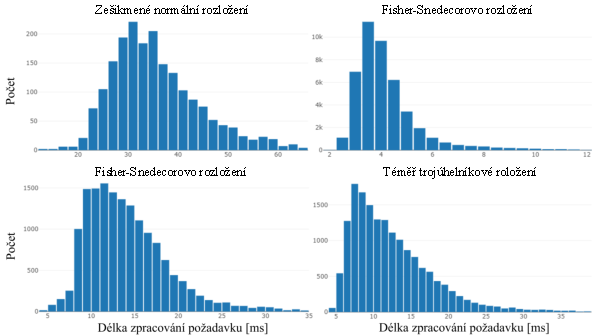
\includegraphics[width=1\textwidth]{obrazky/rqa-data-distribution.pdf}
    \caption{Rozložení délky zpracování požadavků vychází z~normálního rozložení. To však nikdy není čisté, nýbrž kladně zešikmené. Nejčastěji proto připomíná spíše Fisher–Snedecorovo různých volností. V~krajním případě má i tvar trojúhelníku. Rozložení je tedy poměrně různorodé, nicméně vždy se drží mezi normálním a trojúhelníkovým.}
    \label{data-img}
\end{figure}

\section{Detekce anomálií v~délkách zpracování požadavků}
\label{detekce-anomalii-v-delkach-pozadavku}
Jak již bylo zmíněno v podkapitole \ref{anomalie-v-rqa}, cílem je najít shluky mezi outliery. Pro tuto úlohu se nabízí dvě možné řešení. Prvním je aplikace shlukování na celý dataset. Toto řešení však obsahuje zásadní nedostatek, jenž vysvětluje sekce~\ref{shlukova-analyza-nad-kolekci-dat}. Druhou možností je problém rozdělit na~podproblémy. Takový přístup je mnohem flexibilnější a již umožňuje řešit zadanou úlohu. Rozdělení na~podproblémy nejen že rozšiřuje škálu použitelných algoritmů, nýbrž i zjednodušuje hledání jejich parametrů, neboť cíle algoritmů jsou jednodušší. V~první fázi se proto pouze oddělí outliery od~platných dat. Následně se provede shluková analýza nad~těmito outliery. V~posledním kroku se už jen pro každý shluk outlierů rozhodne, zda-li je dostatečně velký pro~označení za~anomálii. Důležité je si však uvědomit, že se nelze zaměřit na~konkrétní data, na~nichž lze perfektně odladit parametry jednotlivých algoritmů. Detekci je potřeba  navrhnout v~obecnosti, aby byla schopna pracovat nad~libovolnými daty popsanými v~předchozí podkapitole.

\subsection{Shluková analýza nad~celou kolekcí dat}
\label{shlukova-analyza-nad-kolekci-dat}
Myšlenka tohoto přístupu je taková, že by se provedlo shlukování nad~celým datasetem a za~anomálie by pak bylo možné považovat krajní shluky. Hlavní výhodou je, že by stačil pouze jeden průchod daty jediným shlukovacím algoritmem. Ten je nutné hledat mezi algoritmy založených na hustotě. Důvodem je dopředná neznalost počtu anomálií, tedy shlukovacích tříd. Zároveň je žádoucí ignorovat osamocené outliery, nebo-li šum, na~což jsou tyto algoritmy dobré. Další důležitou vlastností algoritmu musí být schopnost rozpoznat shluky odlišných hustot, neboť jinak hustý bude hlavní shluk obsahující platná data a jinak pak anomální shluky. Z~algoritmů představených kapitolou~\ref{ml-algoritmy} splňují tyto vlastnosti HDBSCAN a OPTICS. Problém však spočívá v~tom, že není možné najít vhodné parametry vybraných algoritmů. Obrázky~\ref{direct-detection-soft-img} a~\ref{direct-detection-hard-img} znázorňují paradox ve~hledání parametrů. 

\begin{figure}[hbt]
    \centering
    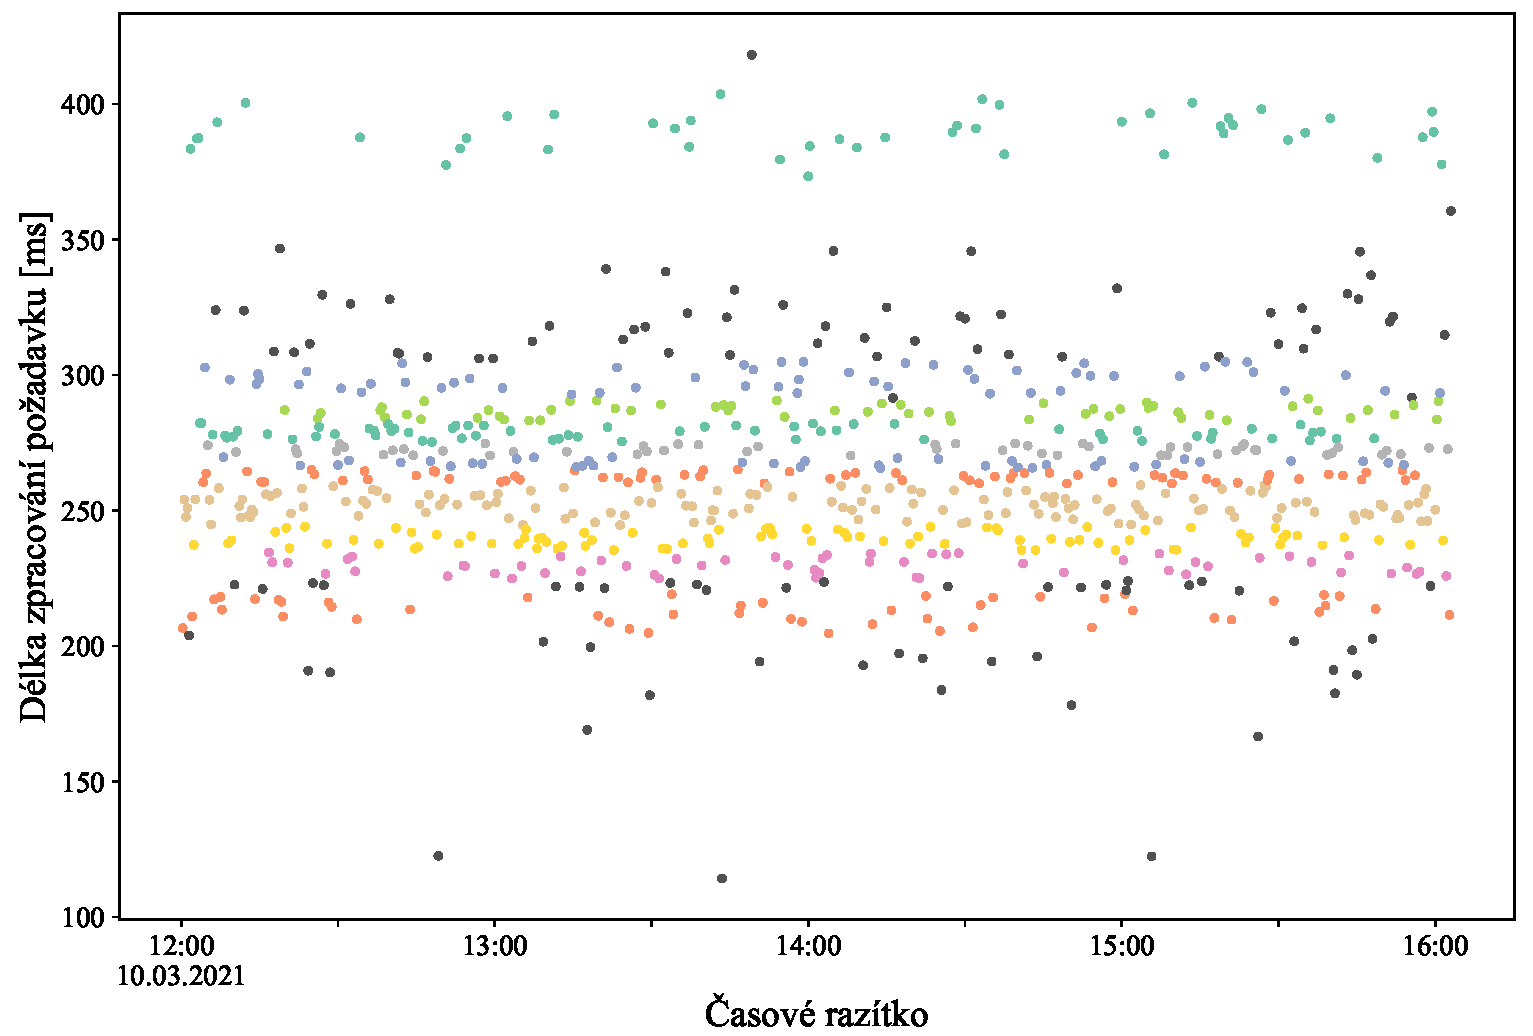
\includegraphics[width=0.88\textwidth]{obrazky/direct-detection-soft.pdf}
    \caption{Nízké nároky na shluk rozštěpí hlavní shluk na~mnoho podshluků.}
    \label{direct-detection-soft-img}
\end{figure}

\begin{figure}[hbt]
    \centering
    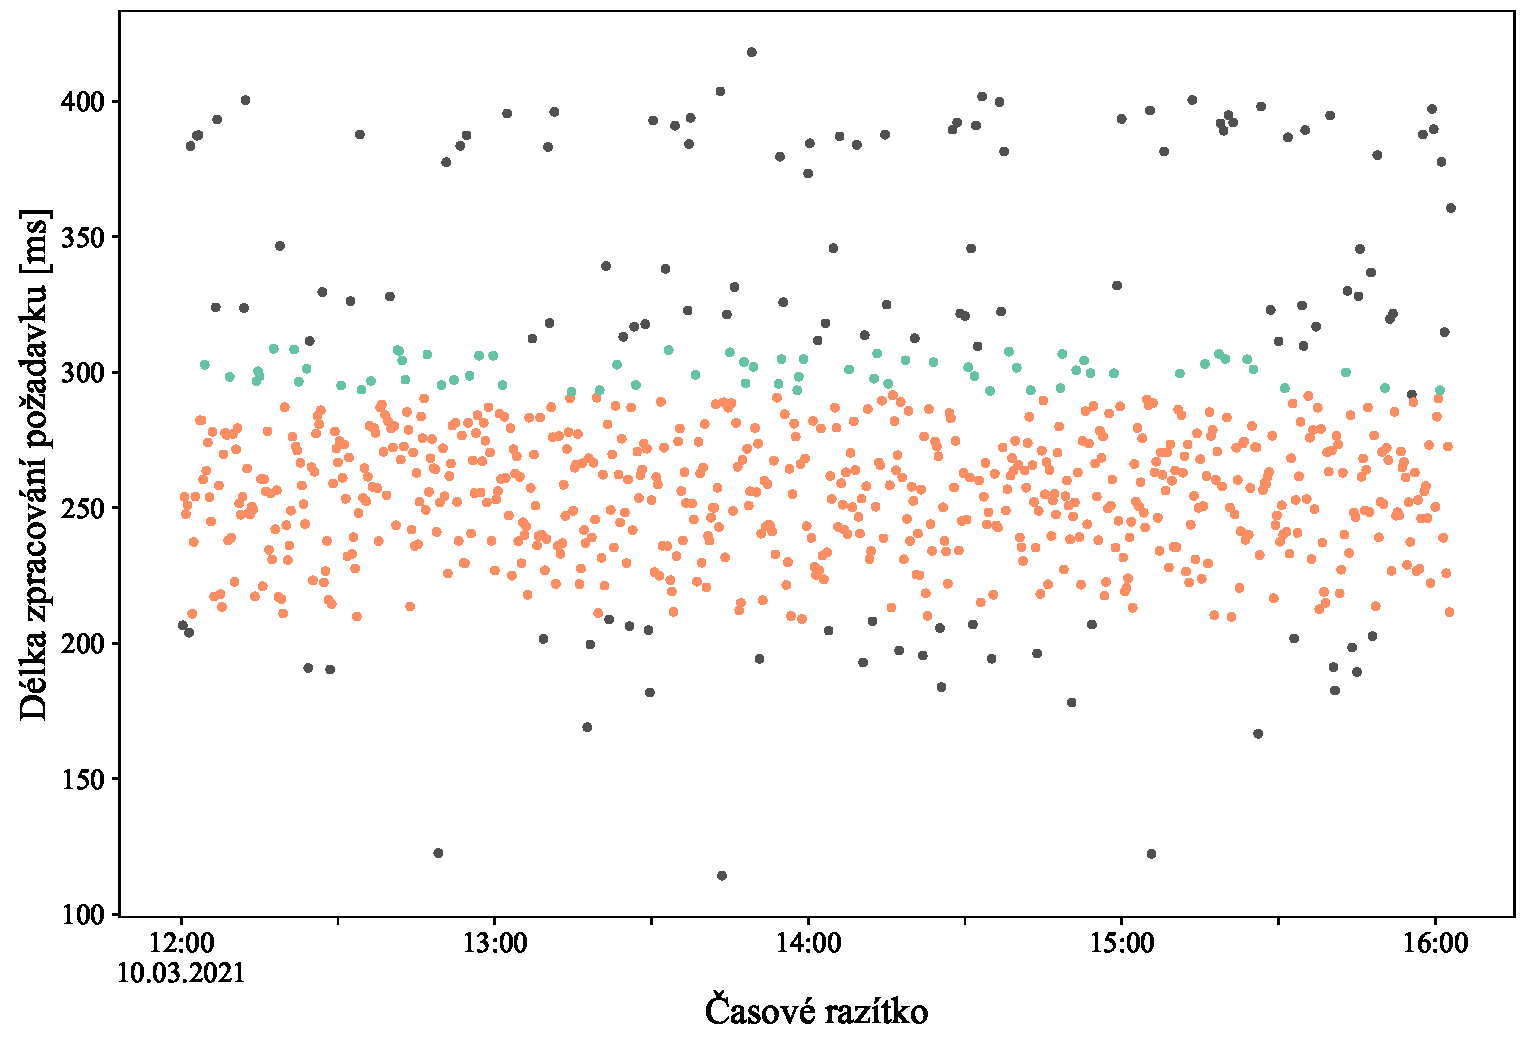
\includegraphics[width=0.88\textwidth]{obrazky/direct-detection-hard.pdf}
    \caption{S~velkými nároky na~shluk není anomálie ani jako shluk rozpoznána.}
    \label{direct-detection-hard-img}
\end{figure}

Na~obou obrázcích lze spatřit anomálii blízko hodnoty 400~ms. Vzhledem k~tomu, že anomální shluky jsou typicky menší a okrajové, je třeba zvolit parametry dostatečně jemně, aby shluky byly rozpoznány. Jak však ukazuje obrázek~\ref{direct-detection-soft-img}, nízké požadavky na~shluk způsobí, že se i hlavní shluk rozštěpí na~mnoho menších, neboť tyto také splňují specifikace shluku. Při~snaze tento problém kompenzovat zpřísňováním požadavků na~shluk nastane situace jako na~obrázku~\ref{direct-detection-hard-img}, na němž již anomální shluk není dostatečně hustý či velký na~to, aby byl za~shluk vůbec považován.

\subsection{Detekce outlierů}
\label{detekce-outlier}
Kapitola~\ref{ml-algoritmy} představila několik algoritmů, které jsou vhodnými kandidáty pro~tento úkol. V~první řadě lze opět použít algoritmy založené na~hustotě. Zde se již hledání parametrů značně zjednoduší, neboť stačí rozlišit jen jeden hlavní shluk platných dat od~šumu. Vzhledem ke~zrušení variability hustoty je výhodné použít základní variantu DBSCAN.

Pro~získání vhodných parametrů byly prováděny experimenty nad~normálním rozložením, jež zobrazuje tabulka~\ref{dbscan-params-table}. Dobrými hodnotami se projevily být číslo~5 pro parametr MinPts a číslo 25 pro~\textepsilon. V~případě, že by dataset obsahoval méně prvků, než dvojnásobek~\textepsilon, tedy~50, je za~\textepsilon~zvolena polovina velikosti datasetu. Vybrané parametry však ještě byly testovány způsobem popsaným v~sekci~\ref{testovani-konkretni-anomalie}, neboť zmíněné experimenty vedly pouze k~získání výchozích hodnot, kolem kterých by se parametry mohly pohybovat. Pro~jiné směrodatné odchylky nebo i jiná rozložení tyto parametry nemusely být optimální. Testování však prokázalo, že nepracují špatně ani s~jinými typy dat, a~proto byly nakonec použity. Obrázek~\ref{dbscan-outlier-detection-img} ukazuje výsledek aplikace DBSCAN algoritmu s~těmito parametry.

\begin{figure}[hbt]
    \centering
    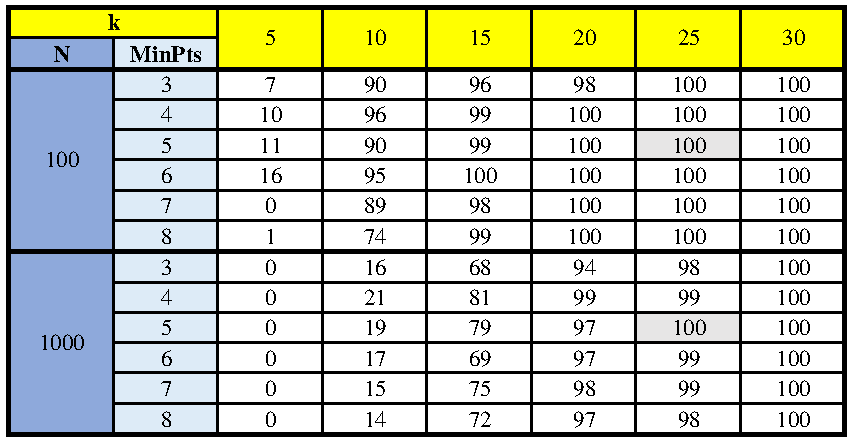
\includegraphics[width=0.935\textwidth]{obrazky/dbscan-params-results.pdf}
    \caption{Tabulka ukazuje výsledky experimentů DBSCAN algoritmu s~různými parametry. Pro~každou kombinaci bylo provedeno 100 pokusů nad~náhodnými daty normálního rozložení se~směrodatnou odchylkou \(\sigma = 15\). Číslo udává počet přijatelných oddělení outlierů od~platných dat zkontrolovaných člověkem. N~zde značí počet prvků rozložení, neboť jinak se algoritmus chová nad~malými a velkými datasety. Písmeno k je \emph{k}-tý soused, vzdálenost k~němuž se použila jako \textepsilon}
    \label{dbscan-params-table}
\end{figure}

\begin{figure}[!hbt]
    \centering
    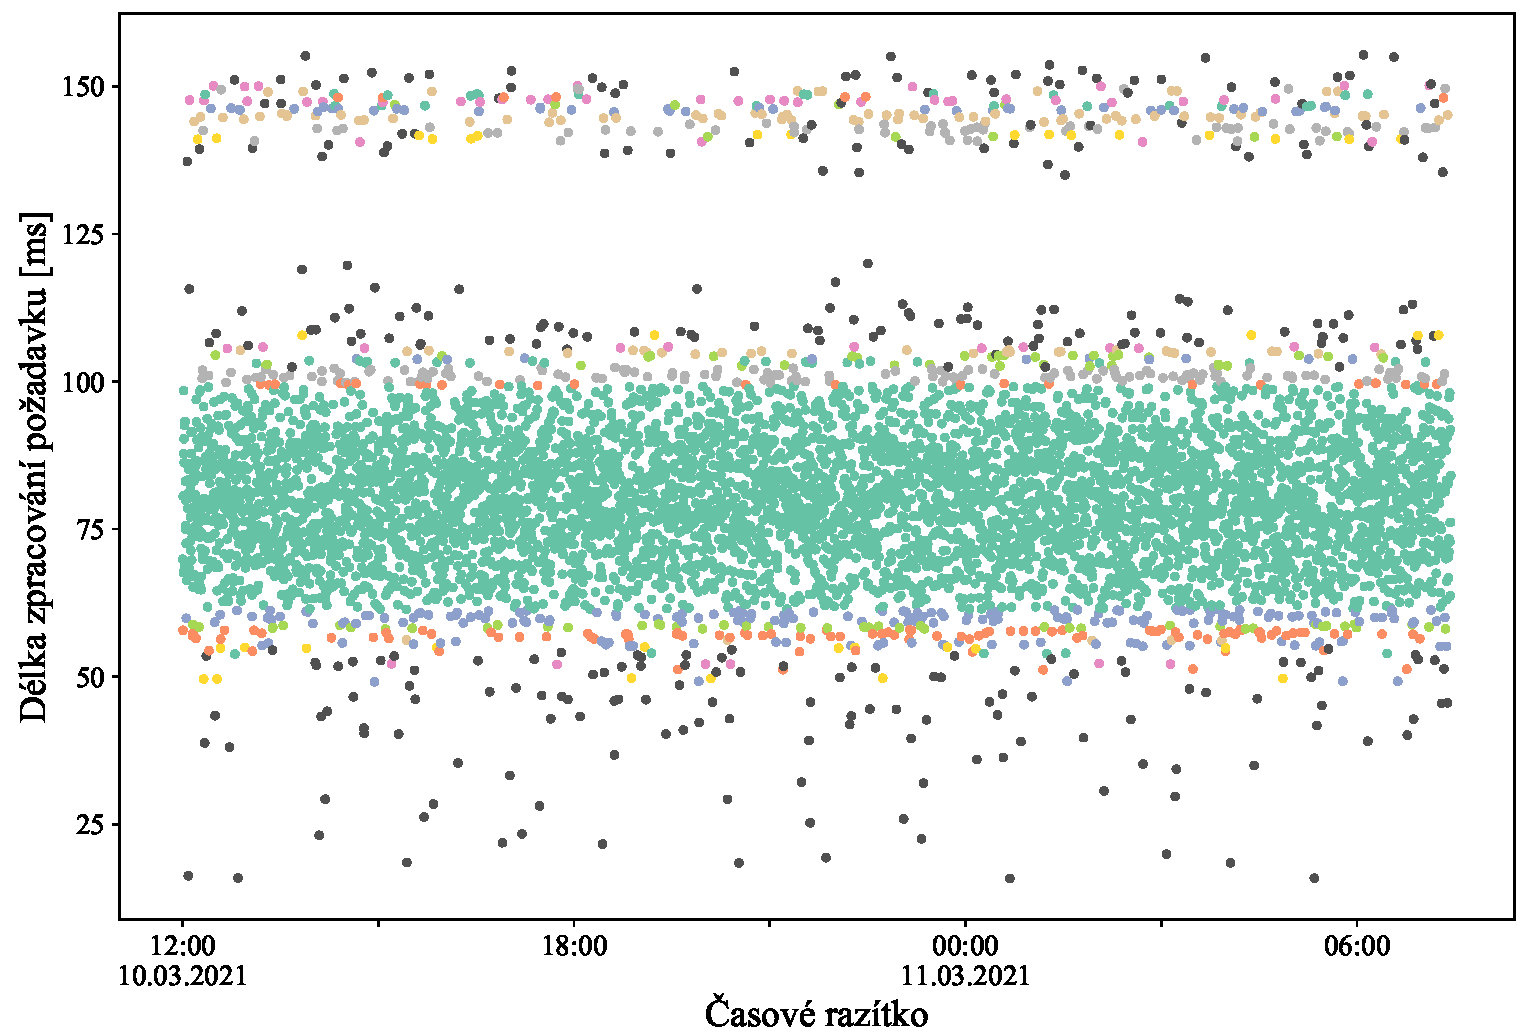
\includegraphics[width=0.935\textwidth]{obrazky/dbscan-outlier-detection.pdf}
    \caption{Za~outliery se v~tomto výsledku DBSCAN algoritmu považuje vše, co nepatří do~hlavního zeleného shluku.}
    \label{dbscan-outlier-detection-img}
\end{figure}

DBSCAN ve~většině případů spolehlivě nalezne hlavní shluk, nicméně jak je vidět, nezahrne velké množství okrajových dat, které by měly být součástí. Přesnost tohoto velmi závisí na konkrétním rozložení. Další problém spočívá v~tom, že u~velmi malých datasetů a ještě s~nepříznivým rozložením občas nenalezne žádné shluky, což není přijatelné.

Další možností je algoritmus Isolation forest, který je přímo optimalizován na~detekci outlierů. Za~parametry byly zvoleny doporučené hodnoty 100 stromů v~lese a 256 vzorků pro~strom~\cite{isolation-forest}. Nalezení hraničního skóre, které by bylo použitelné v~obecnosti, však nebylo možné. Silně totiž závisí na~počtu a hustotě dat. Obrázek~\ref{iForest-outlier-detection-img} zobrazuje případ, kdy je anomálie poměrně hustá a mnoho anomálních dat je považováno za platná. Tento jev je možné odstranit zpřísněním skóre, nicméně přišlo by se tím o~značné množství krajních platných dat. Navíc se nejedná ani o~žádný extrémní případ. Pokud by anomálie byla dostatečně velká a hustší než platná data, budou mít její prvky nižší skóre a nebude možné je vůbec oddělit. Ukázalo se tedy, že Isolation forest by byl vhodný na~odstranění šumu, nicméně nelze ho v~obecnosti využít pro~vytyčení hlavního shluku v~datech.

\begin{figure}[!hbt]
    \centering
    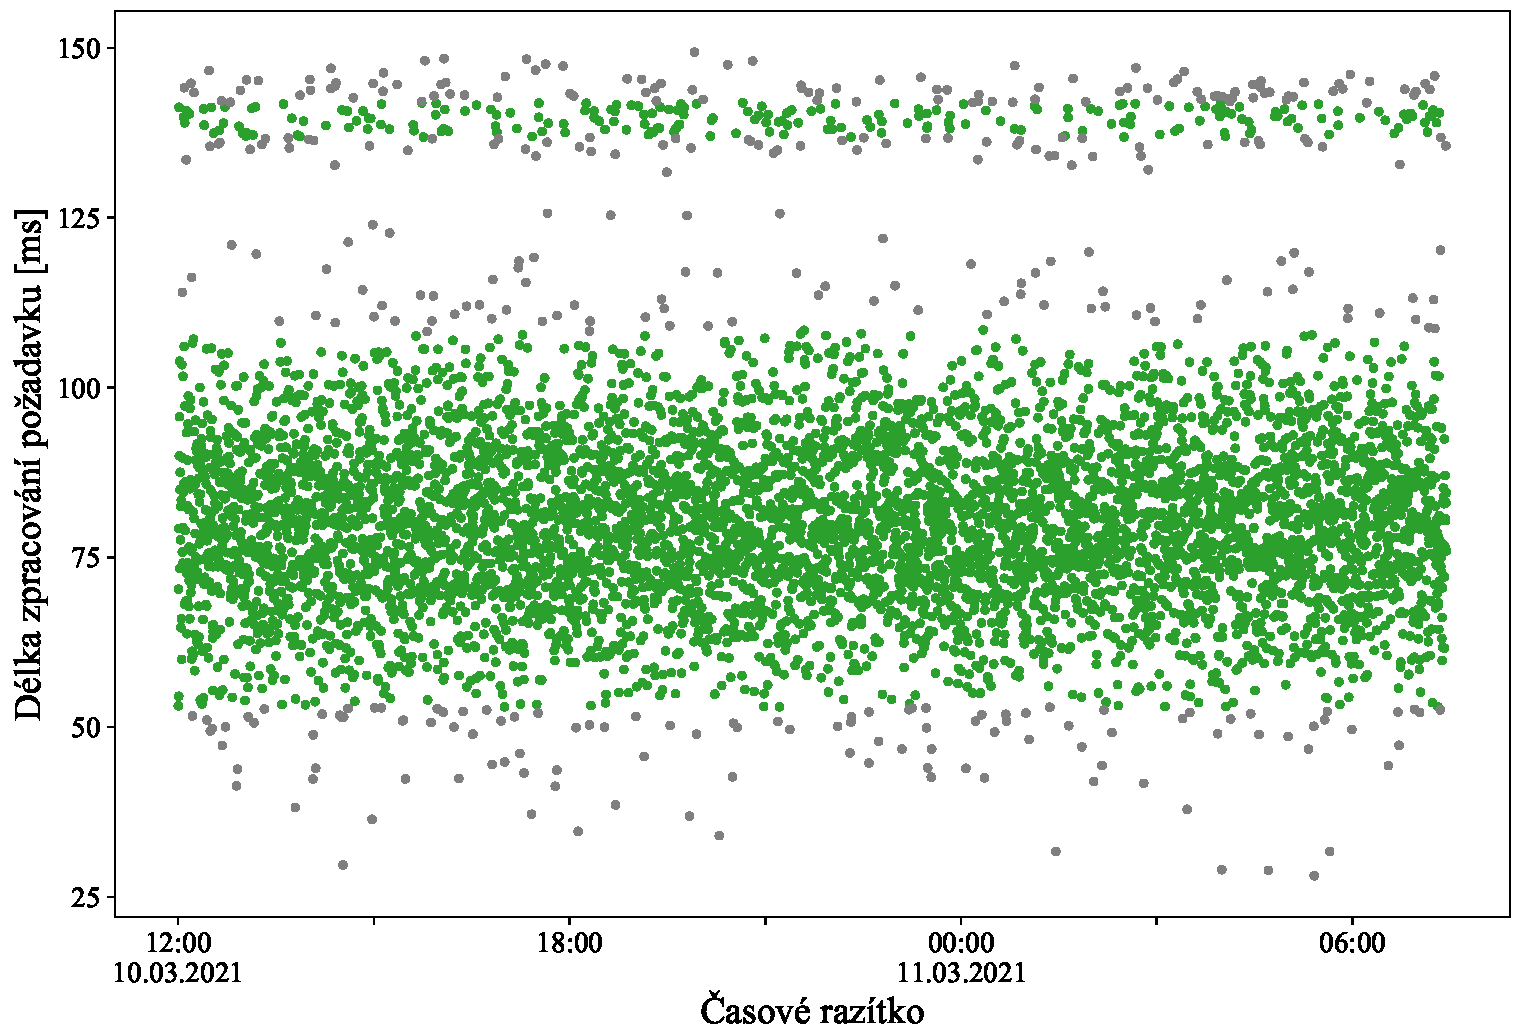
\includegraphics[width=0.88\textwidth]{obrazky/iForest-outlier-detection.pdf}
    \caption{Výsledek algoritmu Isolation forest pro~detekci outlierů}
    \label{iForest-outlier-detection-img}
\end{figure}

Jednodimenzionalita dat a jejich víceméně normální rozložení umožňuje použít i statistickou metodu modifikované z-skóre. Z~výše uvedených je nejrychlejší a vyžaduje pouze jeden parametr. Tím je hraniční skóre, nad~nímž jsou data považována za~outliery. Dobrou hranicí se ukázalo být skóre 2.35, jak lze částečně vypozorovat z~obrázku~\ref{z-score-param-img}. Výchozím hraničním skórem byla hodnota 3, jež bývá často používána~\cite{z-score}. Pro čisté normální rozložení je velmi dobrá, nicméně u~strmějších rozložení (Fisher-Snedecorovo, trojúhelníkové) může zahrnout i mnoho outlierů. Podobným problémem trpí i hodnota 2.5. Přísnější hranice, jakou je třeba číslo 2, se tohoto nedostatku zbavuje, nicméně již zase ořezává dost dat na~druhé straně rozložení. Jako kompromis byla zpočátku zvolena hodnota 2.3, jež byla během testování dle sekce~\ref{testovani-konkretni-anomalie} upravena na 2.35.

\begin{figure}[!hbt]
    \centering
    \subfloat[\centering Normální rozložení]{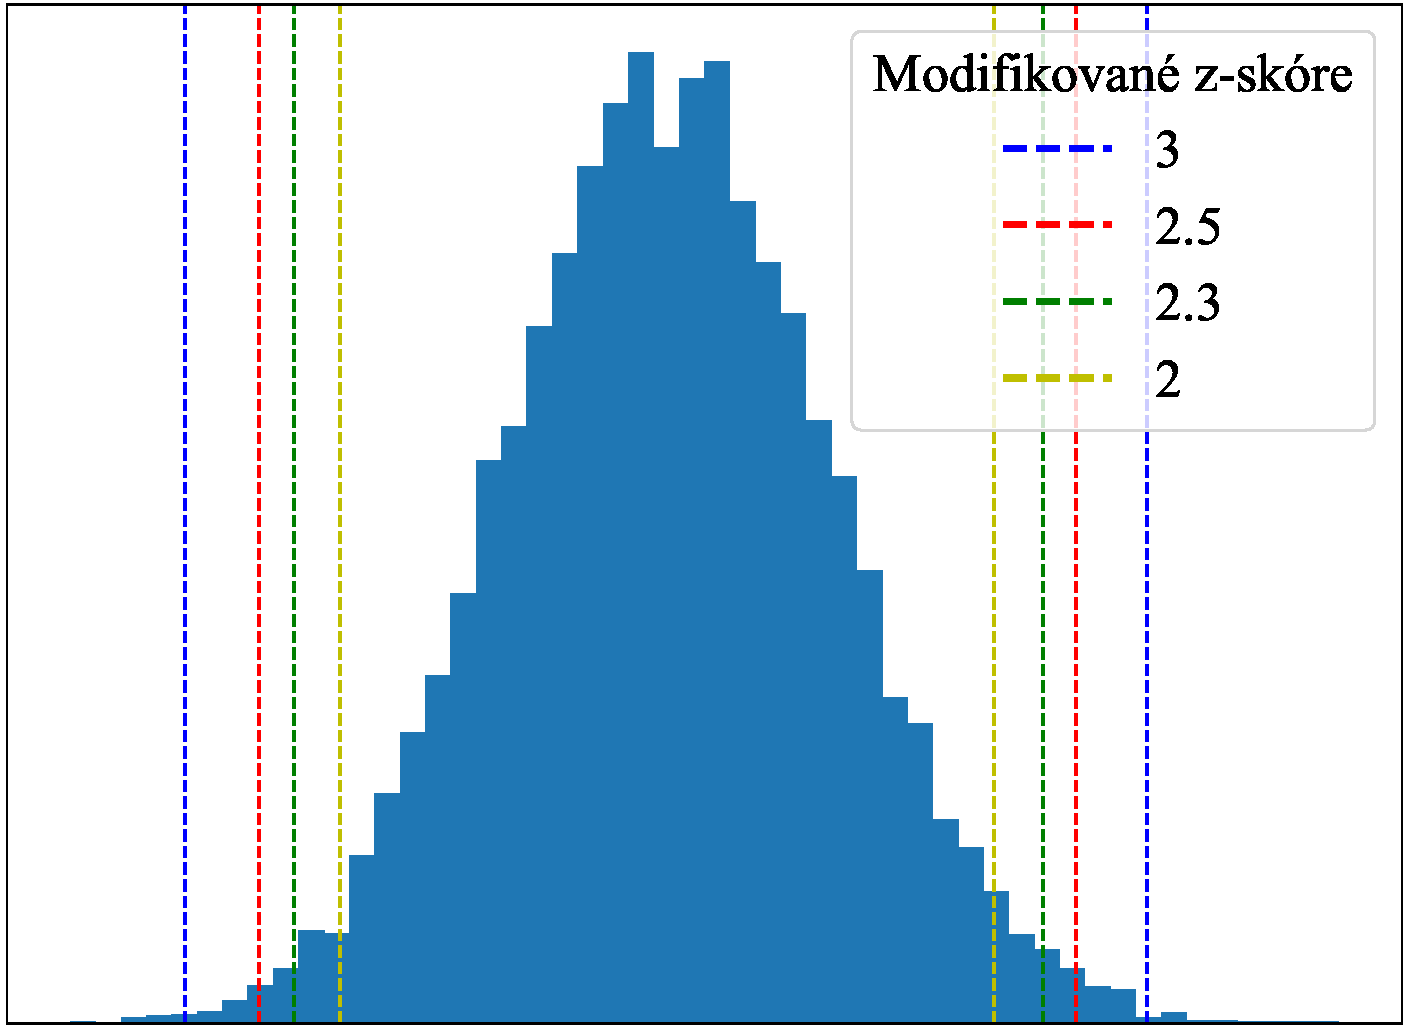
\includegraphics[width=0.49\textwidth]{obrazky/z-score-normal.pdf}}
    \subfloat[\centering Fisher-Snedecorovo rozložení]{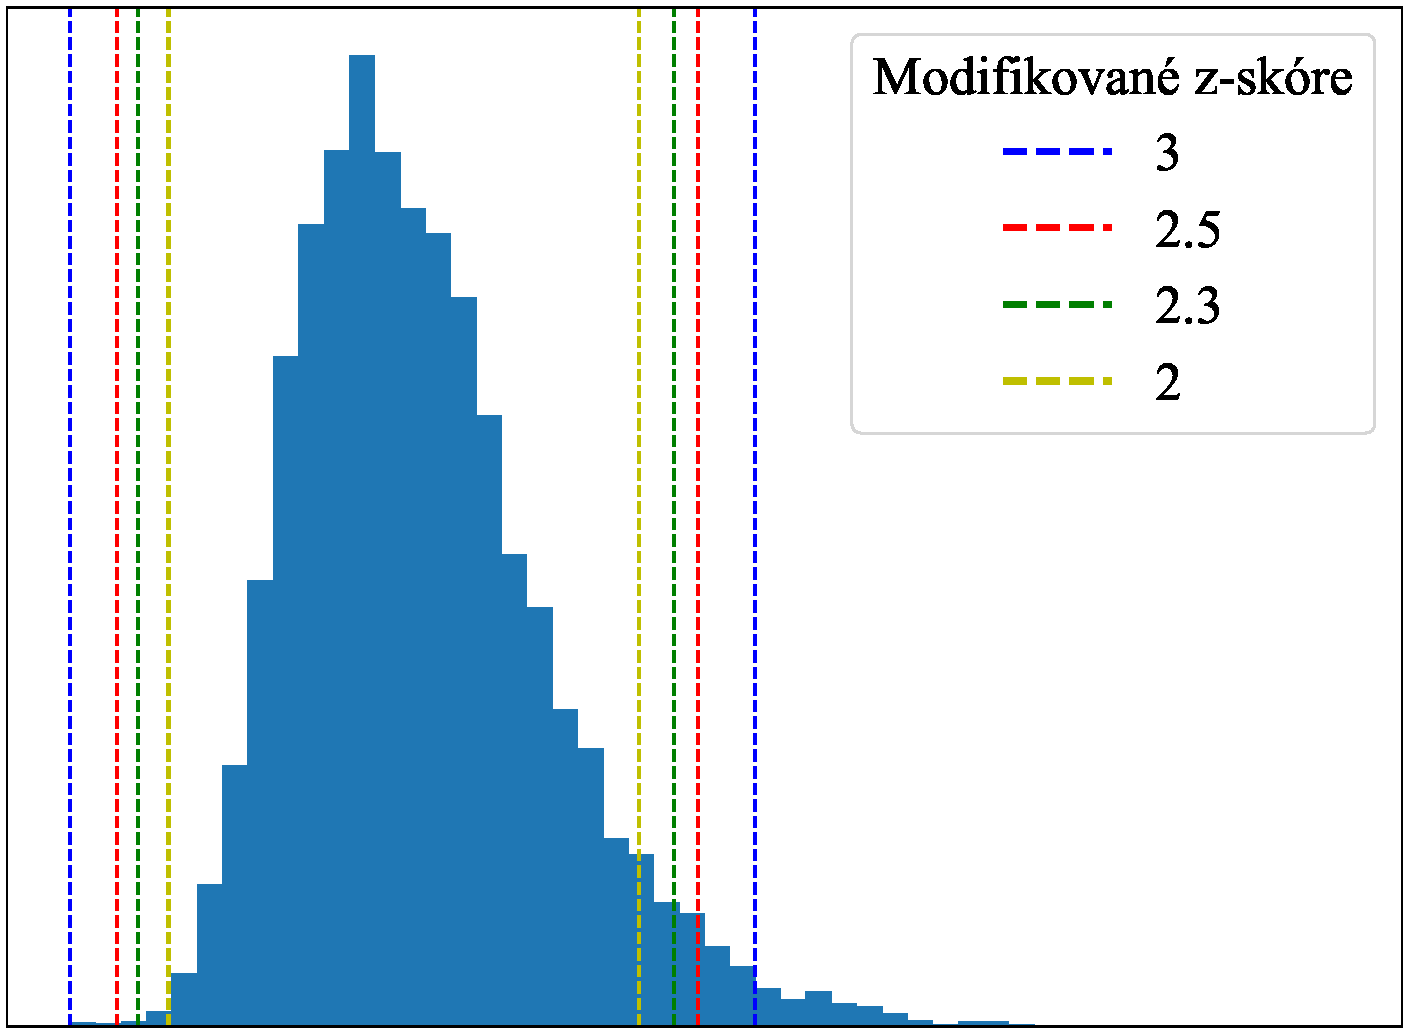
\includegraphics[width=0.49\textwidth]{obrazky/z-score-f.pdf}}
    \qquad
    \subfloat[\centering Trojúhelníkové rozložení]{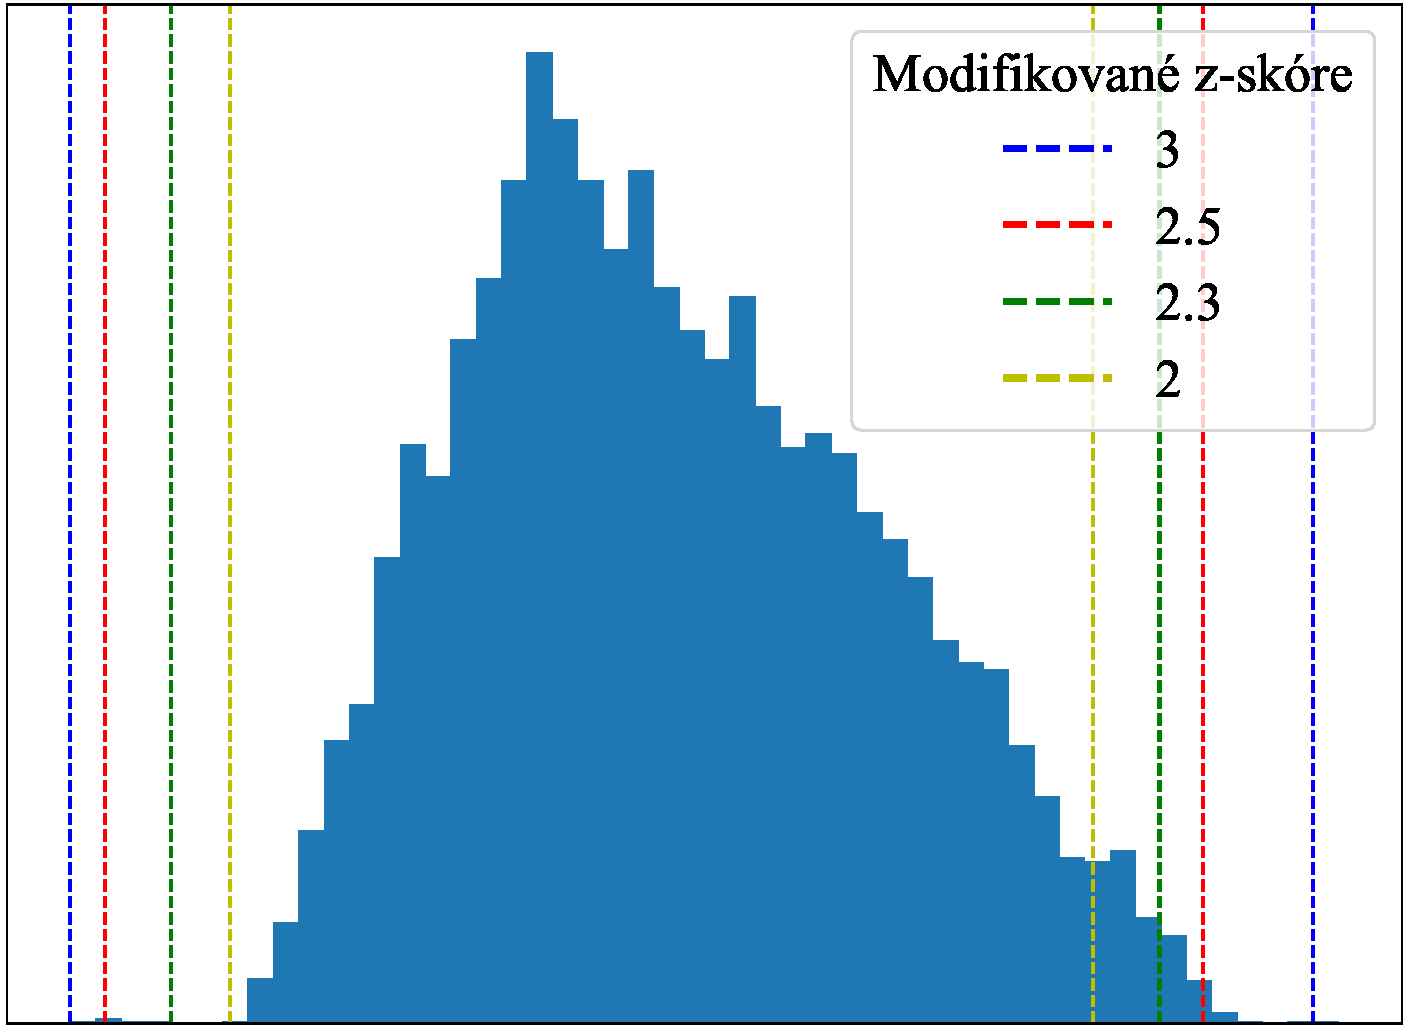
\includegraphics[width=0.49\textwidth]{obrazky/z-score-triangular.pdf}}
    \caption{Hranice modifikovaného z-skóre různých rozložení}
    \label{z-score-param-img}
\end{figure}

Na~obrázku~\ref{modified-zscore-outlier-detection-success-img} pak lze vidět velmi přesné oddělení platných dat a outlierů. Navzdory kvalitním výsledkům však ani metoda modifikovaného z-skóre není perfektní. Čím více se totiž rozložení dat vzdaluje od~normálního, tím větší počet krajních platných dat se odřízne. V~porovnání s jinými algoritmy však toto není nic neobvyklého. Ať už se rozhoduje na~základě hustoty či vzdálenosti, krajní data se přesně nezahrnou téměř nikdy. Pro~požadovanou obecnou detekci dosahuje modifikované z-skóre stále nejpřesnějších výsledků. Nicméně, existuje extrémní případ, kdy selhává i navzdory své značné robustnosti. Jestliže je anomálie velmi velká (třetina datasetu a více) a dostatečně blízko, dokáže ovlivnit i medián a MAD a tím posunou platnou oblast směrem k~anomálii, jako je vyobrazeno na obrázku~\ref{modified-zscore-outlier-detection-fail-img}.

\begin{figure}[!hbt]
    \centering
    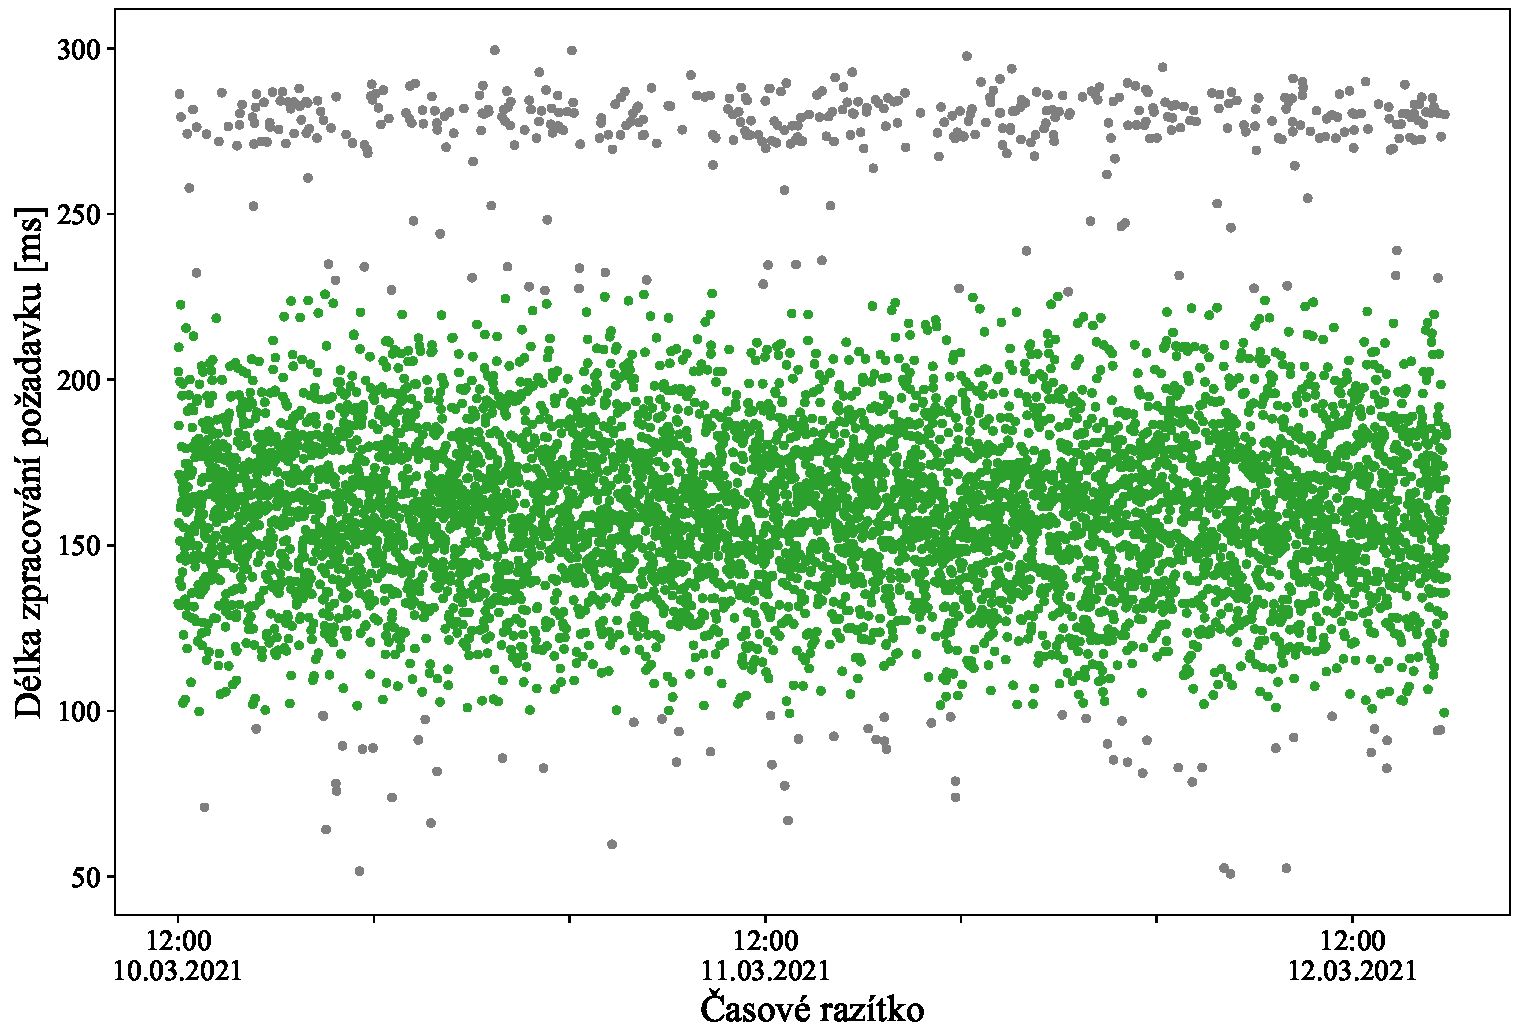
\includegraphics[width=0.935\textwidth]{obrazky/modified-zscore-outlier-detection-success.pdf}
    \caption{Výsledek modifikovaného z-skóre pro detekci outlierů}
    \label{modified-zscore-outlier-detection-success-img}
\end{figure}

\begin{figure}[!hbt]
    \centering
    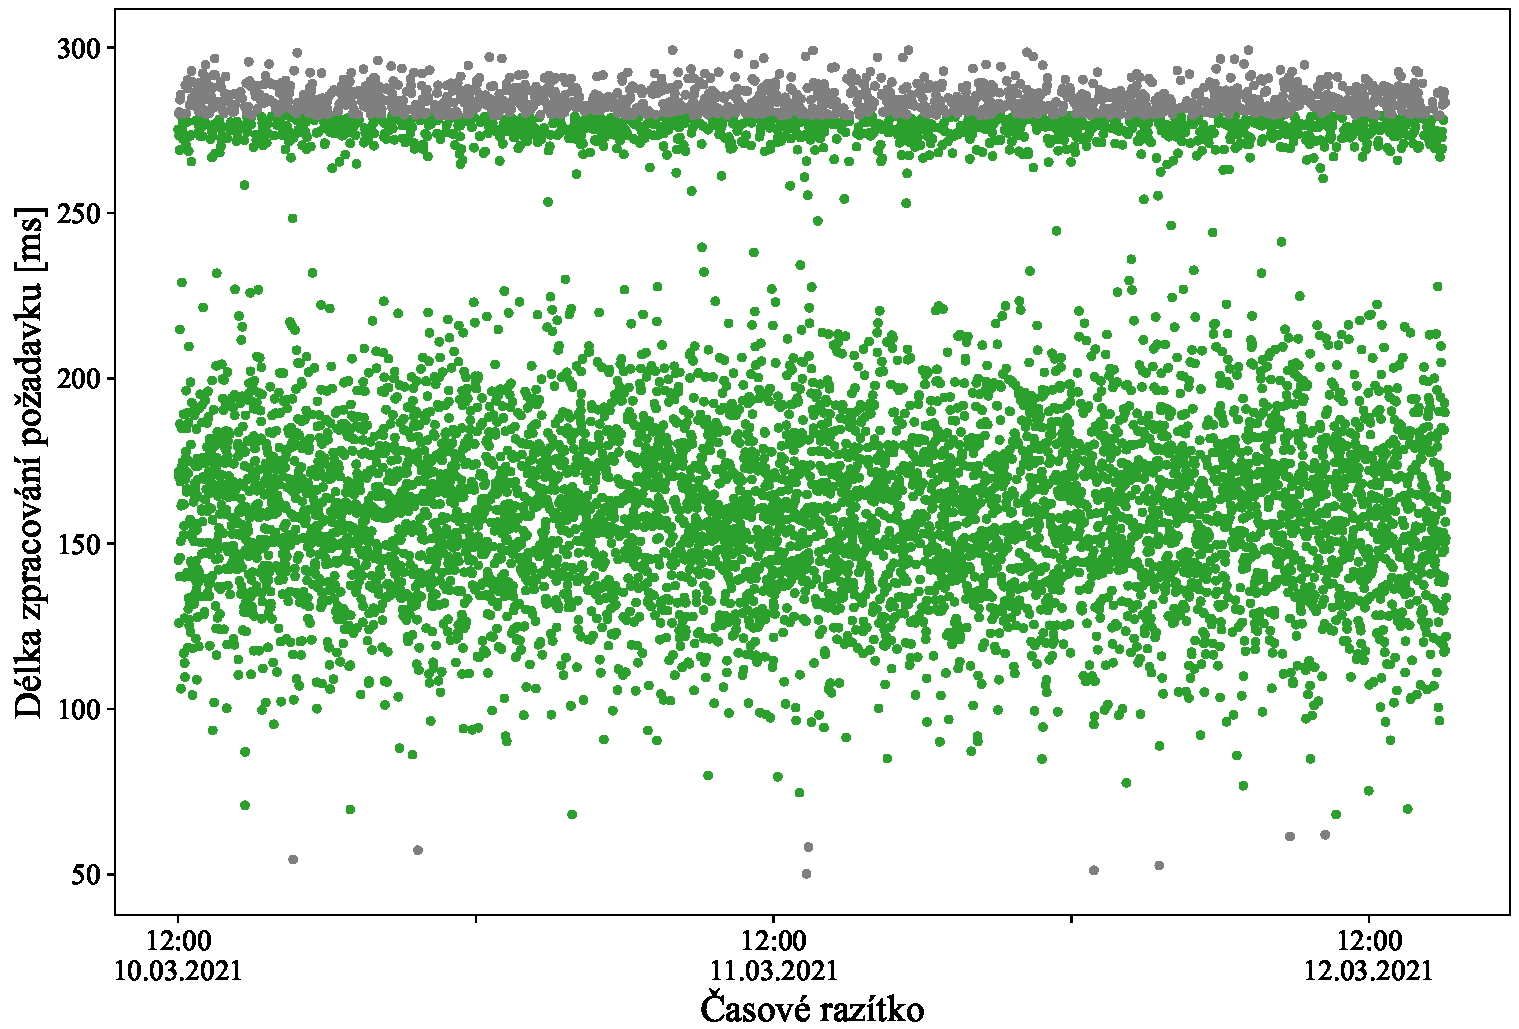
\includegraphics[width=0.935\textwidth]{obrazky/modified-zscore-outlier-detection-fail.pdf}
    \caption{Velká anomálie je schopna posunout medián směrem k~ní a zvětšit MAD natolik, že její část může být považována za platnou.}
    \label{modified-zscore-outlier-detection-fail-img}
\end{figure}

Žádný z~kandidátních algoritmů samostatně nedosahuje optimálních výsledků. Lze však použít jejich kombinaci, konkrétně tedy modifikované z-skóre a DBSCAN. Odstranit problém z~obrázku~\ref{modified-zscore-outlier-detection-fail-img} je možné pomocí parametrů neovlivněných anomálií. V~případě již existujícího referenčního datasetu lze aplikovat samotné modifikované z-skóre. Referenční dataset určuje, kde se nachází platná data, tedy správné centrum v~novém datasetu. Medián a MAD se proto vypočítají z~referenčního datasetu a tyto parametry modifikované z-skóre použije na~nově příchozí data. Referenční dataset se však nejprve musí vytvořit, a~proto je nutné mít způsob nalezení korektního centra datasetu i bez něj. Zde přichází na~řadu DBSCAN. Jak již bylo ukázáno, přestože není moc přesný u~krajních hodnot, hlavní shluk nebo-li hledané centrum datasetu nalézá spolehlivě. Výsledným řešením je tedy nalézt hlavní shluk pomocí DBSCANu, z~něj vypočítat medián a MAD a s~těmito parametry aplikovat modifikované z-skóre na~celý dataset. Tento proces je ukázán na~obrázku~\ref{final-outlier-detection-img}. Modifikované z-skóre rozšíří hlavní shluk nalezený algoritmem DBSCAN, čímž vylepší klasifikaci krajních hodnot. Samo pak díky právě DBSCANu nebude nikdy ovlivněno žádnou anomálií.

\begin{figure}[!hbt]
    \centering
    \subfloat[\centering Nalezení hlavního shluku algoritmem DBSCAN]
    {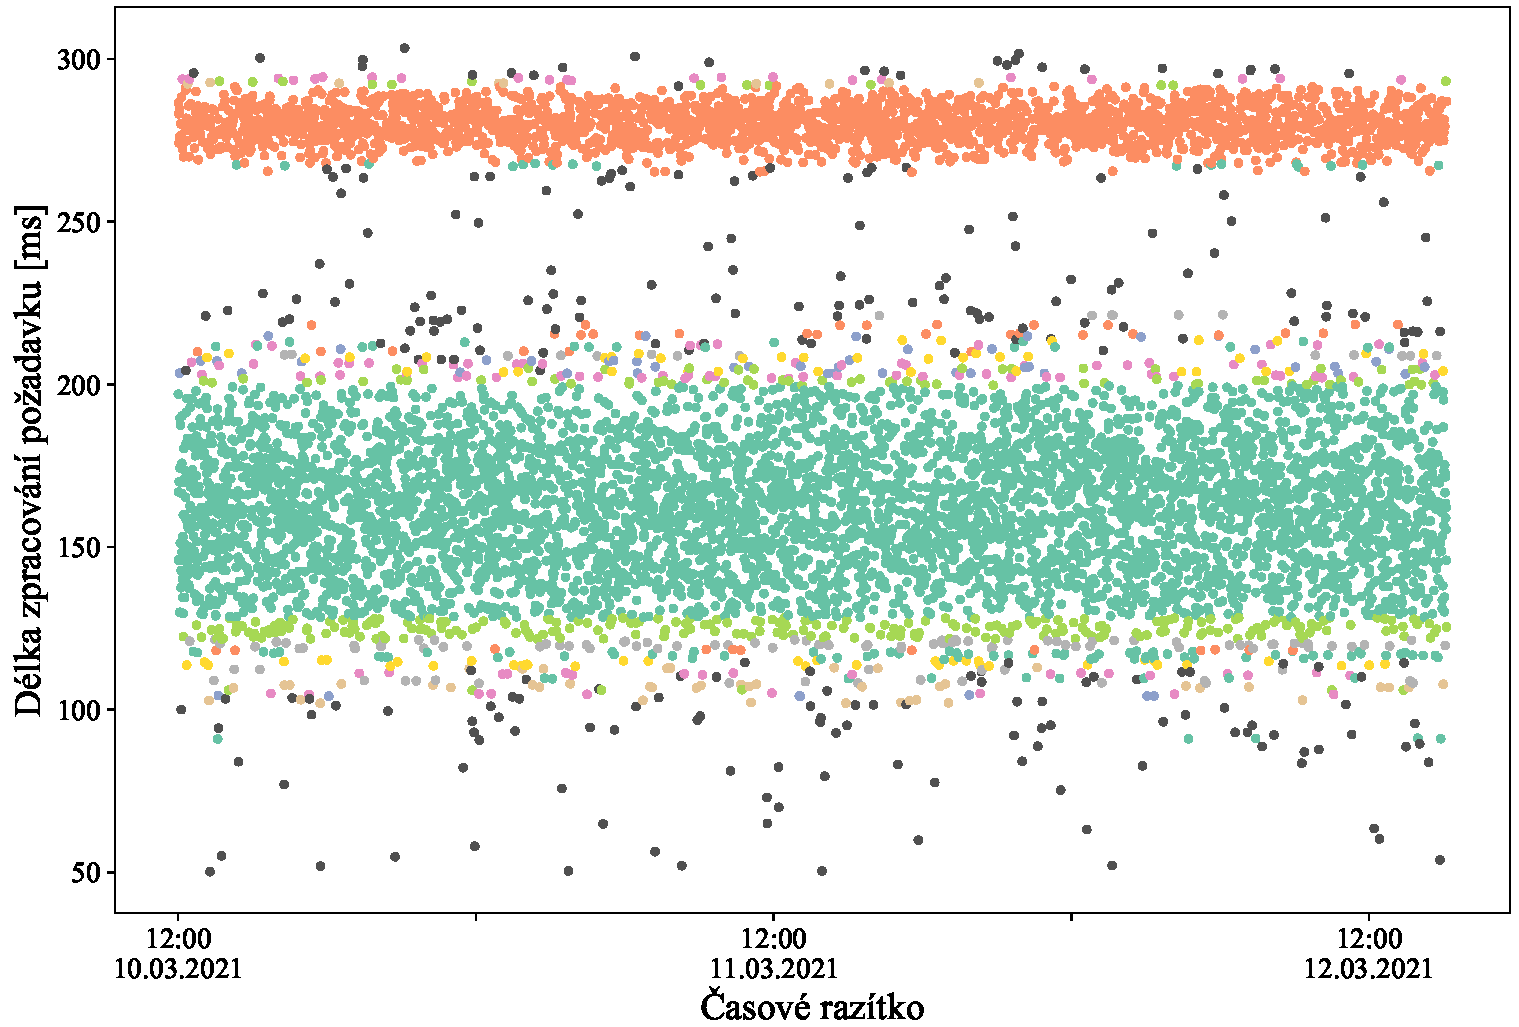
\includegraphics[width=0.935\textwidth]{obrazky/outlier-detection-dbscan-step.pdf}}
    \qquad
    \subfloat[\centering Výsledek modifikovaného z-skóre s~parametry nalezeného hlavního shluku]
    {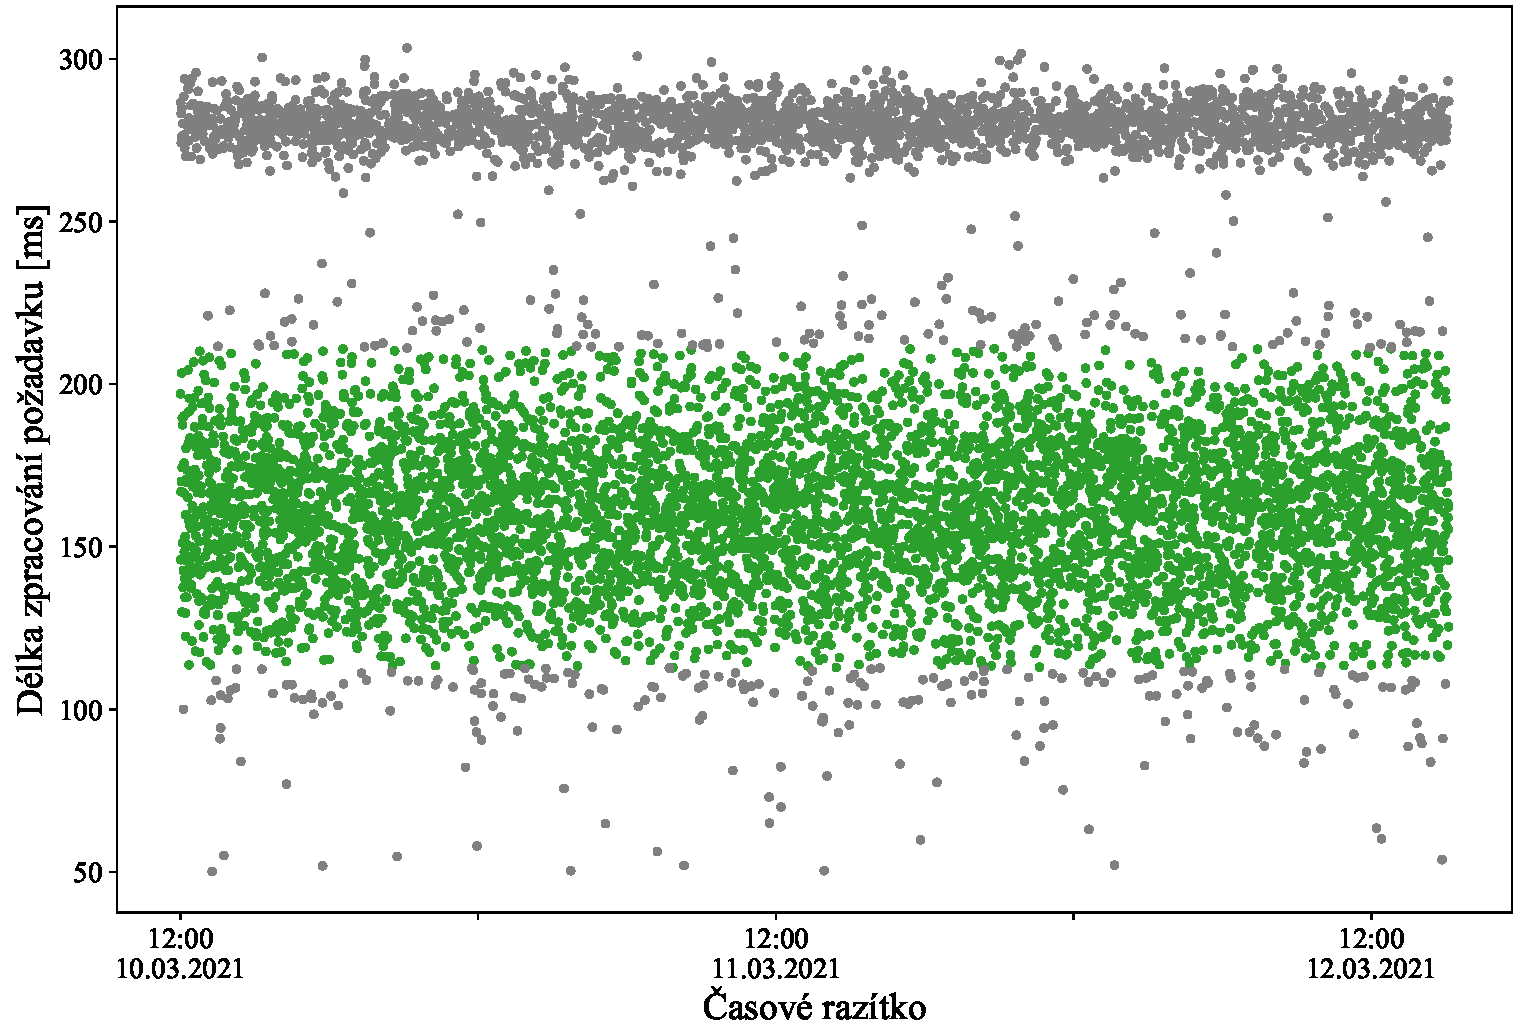
\includegraphics[width=0.935\textwidth]{obrazky/outlier-detection-zscore-step.pdf}}
    \caption{Výsledný postup detekce outlierů kombinací algoritmu DBSCAN a modifikovaného z-skóre}
    \label{final-outlier-detection-img}
\end{figure}

\subsection{Shluková analýza nad outliery}
K~nalezení shluků mezi outliery je možné opět použít HDBSCAN či OPTICS. Nyní je již v~porovnání s~postupem v~sekci~\ref{shlukova-analyza-nad-kolekci-dat} hledání parametrů mnohem jednoduší, neboť nehrozí chybné shlukování platných dat. Z~těchto dvou algoritmů byl vybrán HDBSCAN, neboť je rychlejší, má na~rozdíl od~OPTICS implementaci na~.NET platformě a i hledání parametrů se ukázalo být snazší. Parametr minimální velikosti shluku je poměrně intuitivní. Vzhledem k tomu, že outliery tvoří již značně menší dataset a přebytečné shluky lze jednoduše ignorovat, je lepší mít menší nároky na~shluk. Za~limit proto bylo vybráno alespoň~5~\% z~celkového počtu outlierů. Parametr~\emph{k}, tedy index souseda pro~výpočet vzdálenosti vzájemné dosažitelnosti, zjednodušeně udává hranici mezi šumem a shlukem. Čím vyšší~\emph{k}, tím spíše se bod identifikuje jako šum místo člena shluku~\cite{hdbscan}. Opět protože je shluky spíše žádoucí nalézat, je dobré přiřadit tomuto parametru nižší hodnotu, jíž zpočátku bylo~5~\% z~minimální velikosti shluku. V~průběhu testování se však tato hodnota postupně navýšila až na~10~\%. Vzhledem k~procentuálním výpočtům je nutné určit nepřekročitelná minima těchto parametrů, jimiž jsou~3 pro~minimální velikost shluku a 1 pro~\emph{k}. Na~obrázku~\ref{anomaly-detection-hdbscan-img} je ukázán výsledek HDBSCAN algoritmu nad~outliery.

\begin{figure}[hbt]
    \centering
    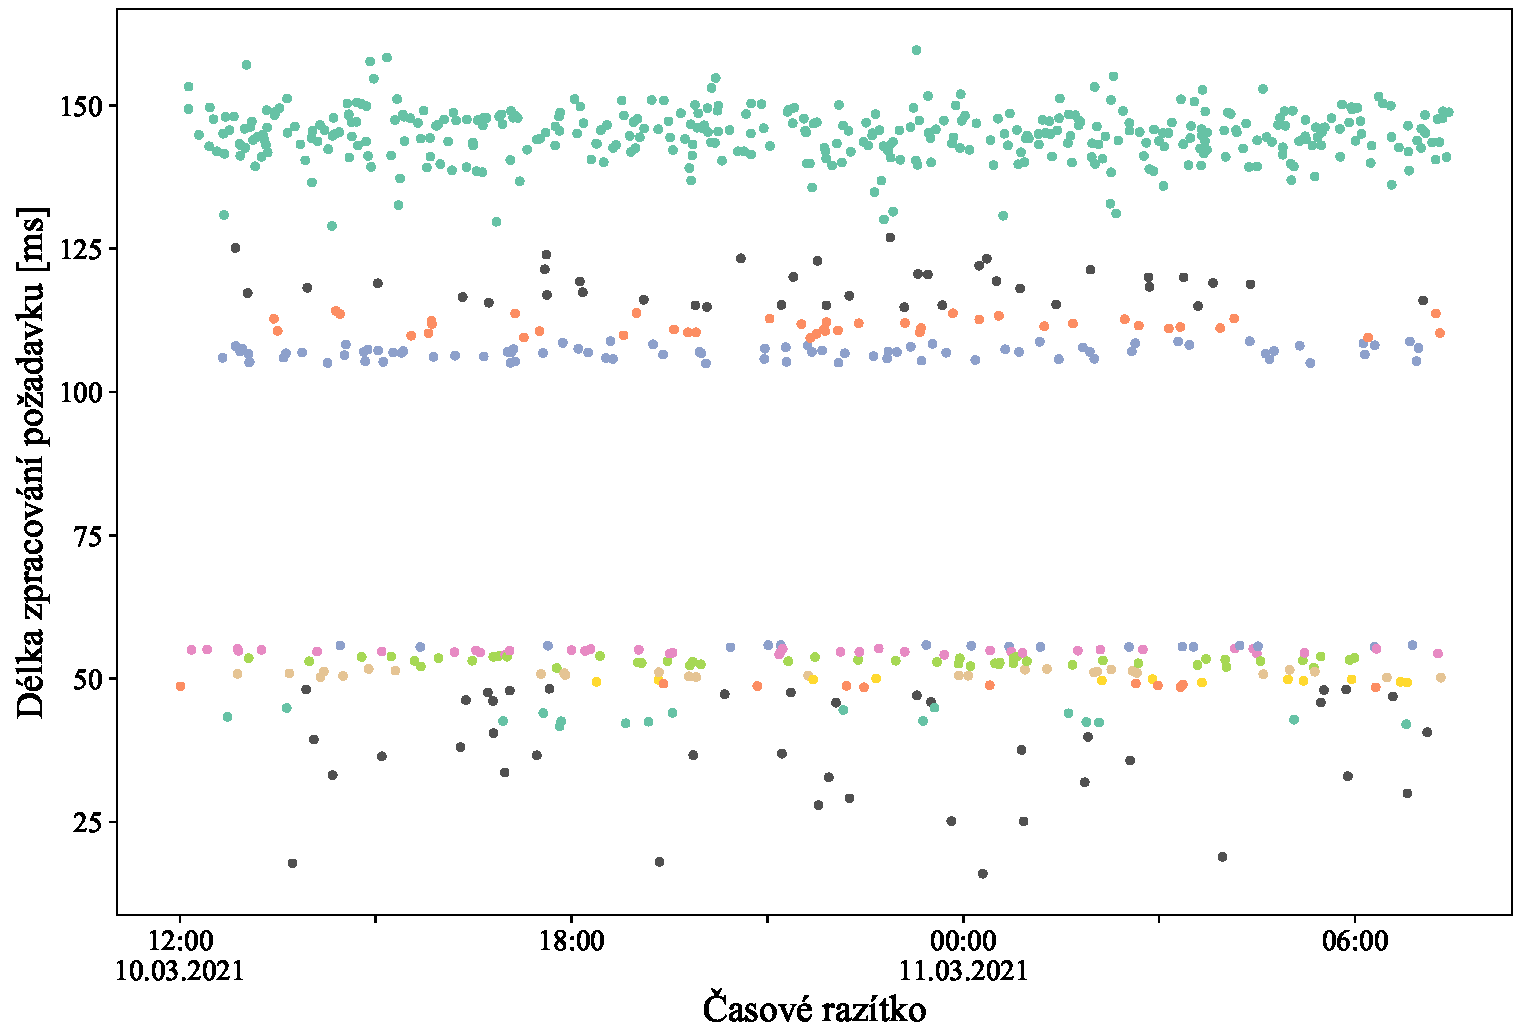
\includegraphics[width=0.88\textwidth]{obrazky/anomaly-detection-hdbscan.pdf}
    \caption{Shluky outlierů nalezené algoritmem HDBSCAN}
    \label{anomaly-detection-hdbscan-img}
\end{figure}

Ukázalo se, že HDBSCAN pracuje poměrně dobře s~ohledem na~obecnost a kvalita výsledků roste s~počtem dat. Na~druhou stranu při~méně než~30 outliery zcela selhává a většinou nenalezne nic. U~takto málo dat ovšem nemá ani cenu řešit různorodost hustot, a~proto lze použít DBSCAN, jenž je dokáže shlukovat kvalitně. Jako MinPts se používá hodnota 3 kvůli co nejmírnějším požadavkům na~shluk. Za~\textepsilon~je volen medián ze~vzdáleností ke~\emph{k}-tému sousedu, kde \emph{k} je polovina z~celkového počtu outlierů. To zajistí relativně velký rozptyl, tedy zvýší šanci na~vytvoření shluku. Jelikož outliery mohou být velmi rozptýleny, je tato vzdálenost shora omezena na~čtvrtinu rozptylu platných dat, aby se nevytvářely příliš široké a řídké shluky.

Navzdory přijatelným výsledkům však nelze nalezené shluky považovat za~konečné. Z~důvodu požadavku na~obecnost detekce jsou tyto podobně jako ty od~DBSCANu v~předchozí sekci jen hrubé. Na~konkrétním příkladu z~obrázku~\ref{anomaly-detection-hdbscan-img} je anomální shluk nalezen celý, nicméně přirozené krajní outliery zde nezobrazených platných dat vytvořily zbytečně mnoho malých shluků, což se v~jiném případě může stát i anomálnímu shluku. V~závislosti na~tvaru a počtu dat budou tyto výsledky vždy jiné, občas zcela přesně rozdělené na~správné shluky, jindy zase až příliš jemně.

Problém příliš malých shluků je řešen sloučením blízkých sousedů. Každý shluk je poměřen s~jeho následujícím sousedem a kontroluje se, zda-li nejsou blízko sebe. Vzájemná blízkost se měří následovně. Překrývají-li se dva shluky s~ohledem na~pravidlo 3-sigma, tedy platí-li nerovnice \(median_1 + 3\sigma_1 > median_2 - 3\sigma_2\), shluky jsou blízké. Během testování se občas ukázaly případy, kdy byl nějaký shluk rozdělen na~mnoho menších shluků příliš úzkých na~sloučení na~základě 3-sigma. Musela se proto zavést i fixní minimální vzdálenost mezi~2 shluky. Idea spočívala v~tom vzít nízké procento rozptylu platných dat, jež se v~průběhu testování ustálilo na hodnotě~2.5~\%. Je-li tedy vzdálenost mezi dvěma shluky menší než~2.5~\% rozptylu platných dat, jsou taktéž blízké.

Druhou podmínkou pro~sloučení je vedle blízkosti i podobná hustota. Z~obou shluků se vezme polovina sousedící s~druhým shlukem, tedy pravá polovina levého shluku a levá polovina pravého shluku. Z~každé se spočítá medián vzdáleností ke~\emph{k}-tému sousedu, kde~\emph{k} je menší z~hodnot 10 a polovina velikosti dané poloviny shluku. Co se zvolí za~hodnotu \emph{k}~není příliš významné, neboť vzdálenost k~dalším sousedům roste s~\emph{k} úměrně díky rovnoměrné hustotě shluku zajištěné algoritmem HDBSCAN. Hodnota~10 byla zvolena proto, že u~vyšších by se již jen zbytečně počítalo více vzdáleností a naopak nízké jednotky by přece jen mohly trpět lokálními výkyvy. Tato vzdálenost ke~\emph{k}-tému sousedu tak udává jistou míru hustoty a je-li jedna více než 2.5krát větší než druhá, tedy jeden shluk je výrazně hustší než druhý, není splněna podmínka podobné hustoty. Hodnota~2.5 byla zvolena na~základě porovnání různých hustot rovnoměrných rozložení jako zobrazuje obrázek~\ref{porovnani-hustot-img}. Dvojnásobná hustota ještě poměrně splývá, trojnásobná již však vyčnívá příliš. Hodnota~2.5 se ukázala být dobrou kompromisní hranicí. Ve~výsledku se sloučí pouze ty sousední shluky, které jsou blízko sebe a mají podobnou hustotu. Celý proces se iterativně opakuje, dokud existují slučitelné shluky. Obrázek~\ref{anomaly-detection-merged-clusters-img} zobrazuje výsledek celého procesu shlukování outlierů.

\begin{figure}[!hbt]
    \centering
    \subfloat[\centering 2x větší hustota]{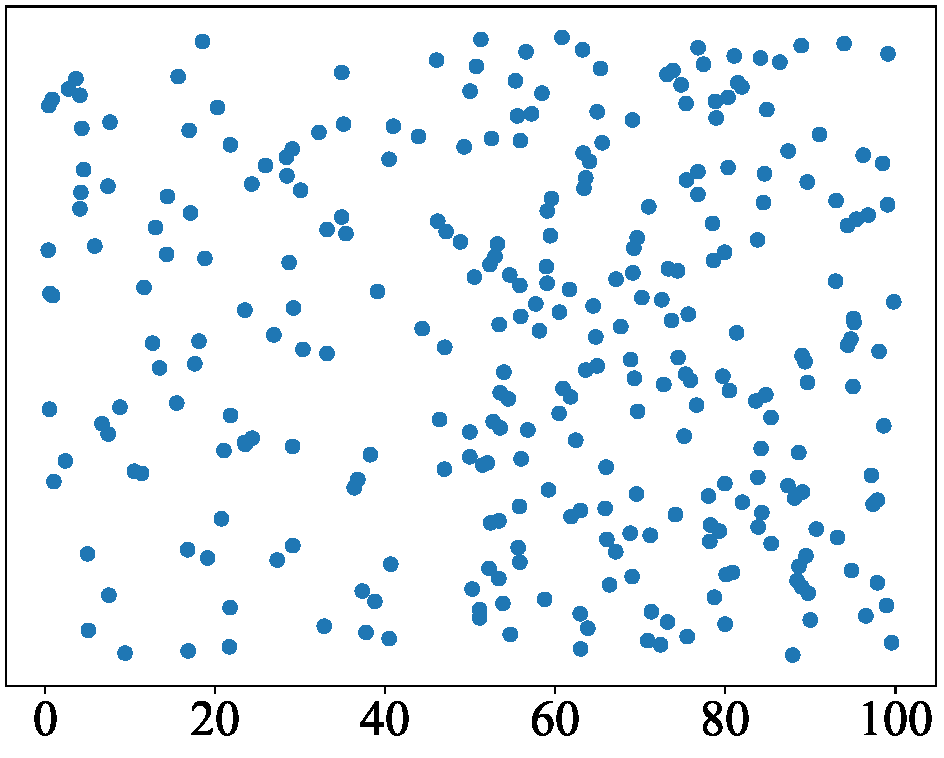
\includegraphics[width=0.32\textwidth]{obrazky/density-2x.pdf} }
    \subfloat[\centering 2.5x větší hustota]{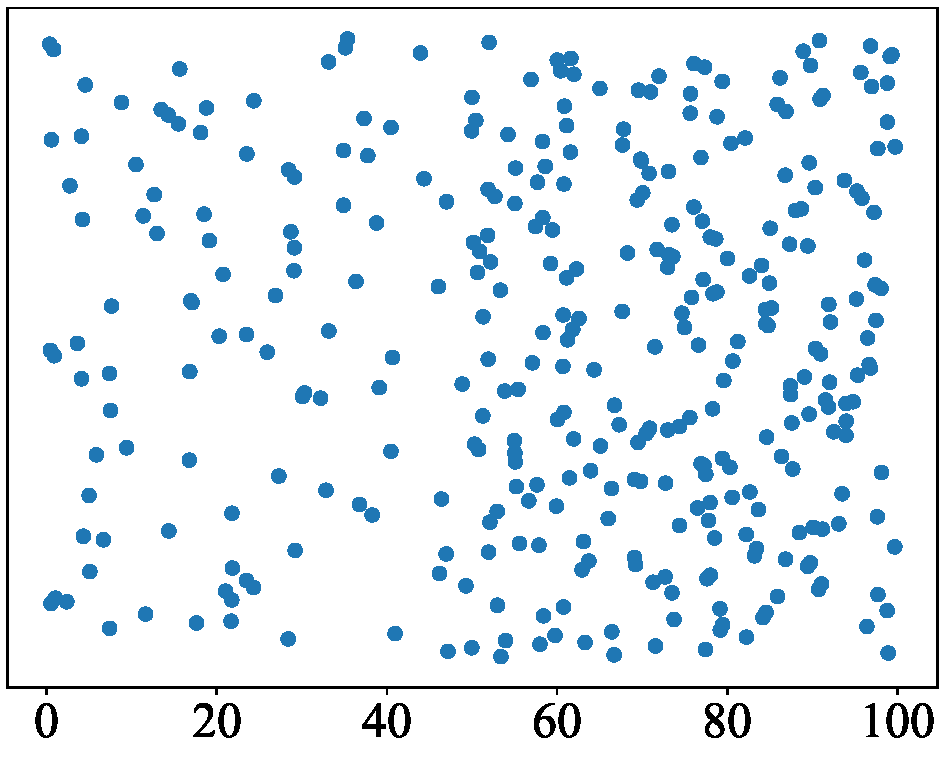
\includegraphics[width=0.32\textwidth]{obrazky/density-2.5x.pdf} }
    \subfloat[\centering 3x větší hustota]{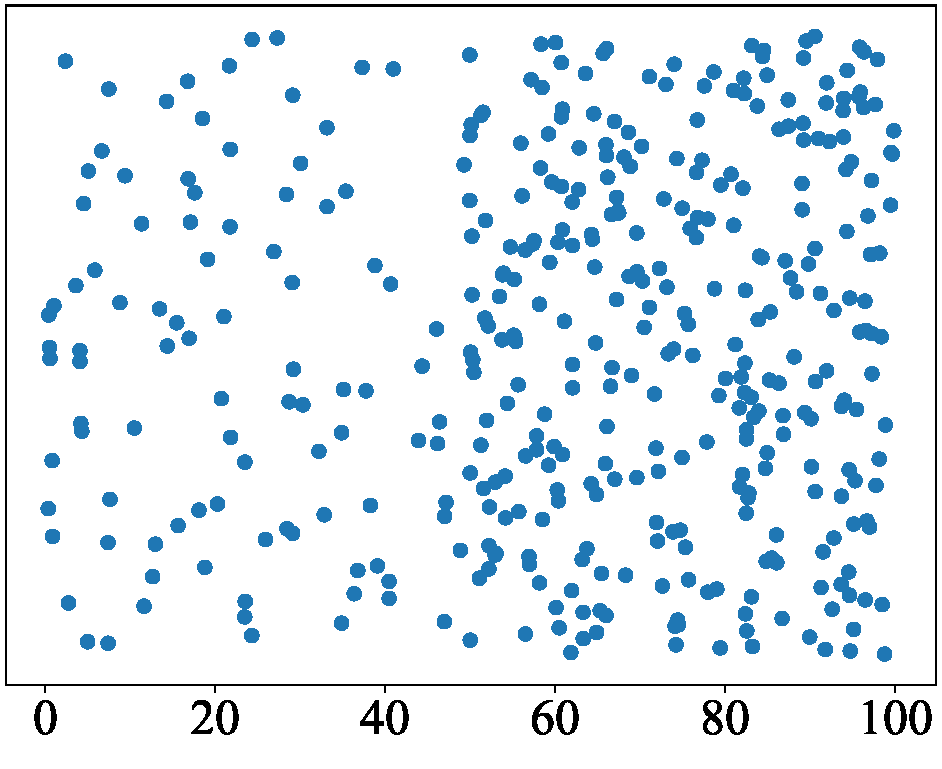
\includegraphics[width=0.32\textwidth]{obrazky/density-3x.pdf} }
    \caption{Porovnání rozložení s~odlišnou hustotou. V~intervalu 0-50 je porovnávané rozložení, mezi 50-100 jsou vždy hustší rozložení.}
    \label{porovnani-hustot-img}
\end{figure}

\begin{figure}[!hbt]
    \centering
    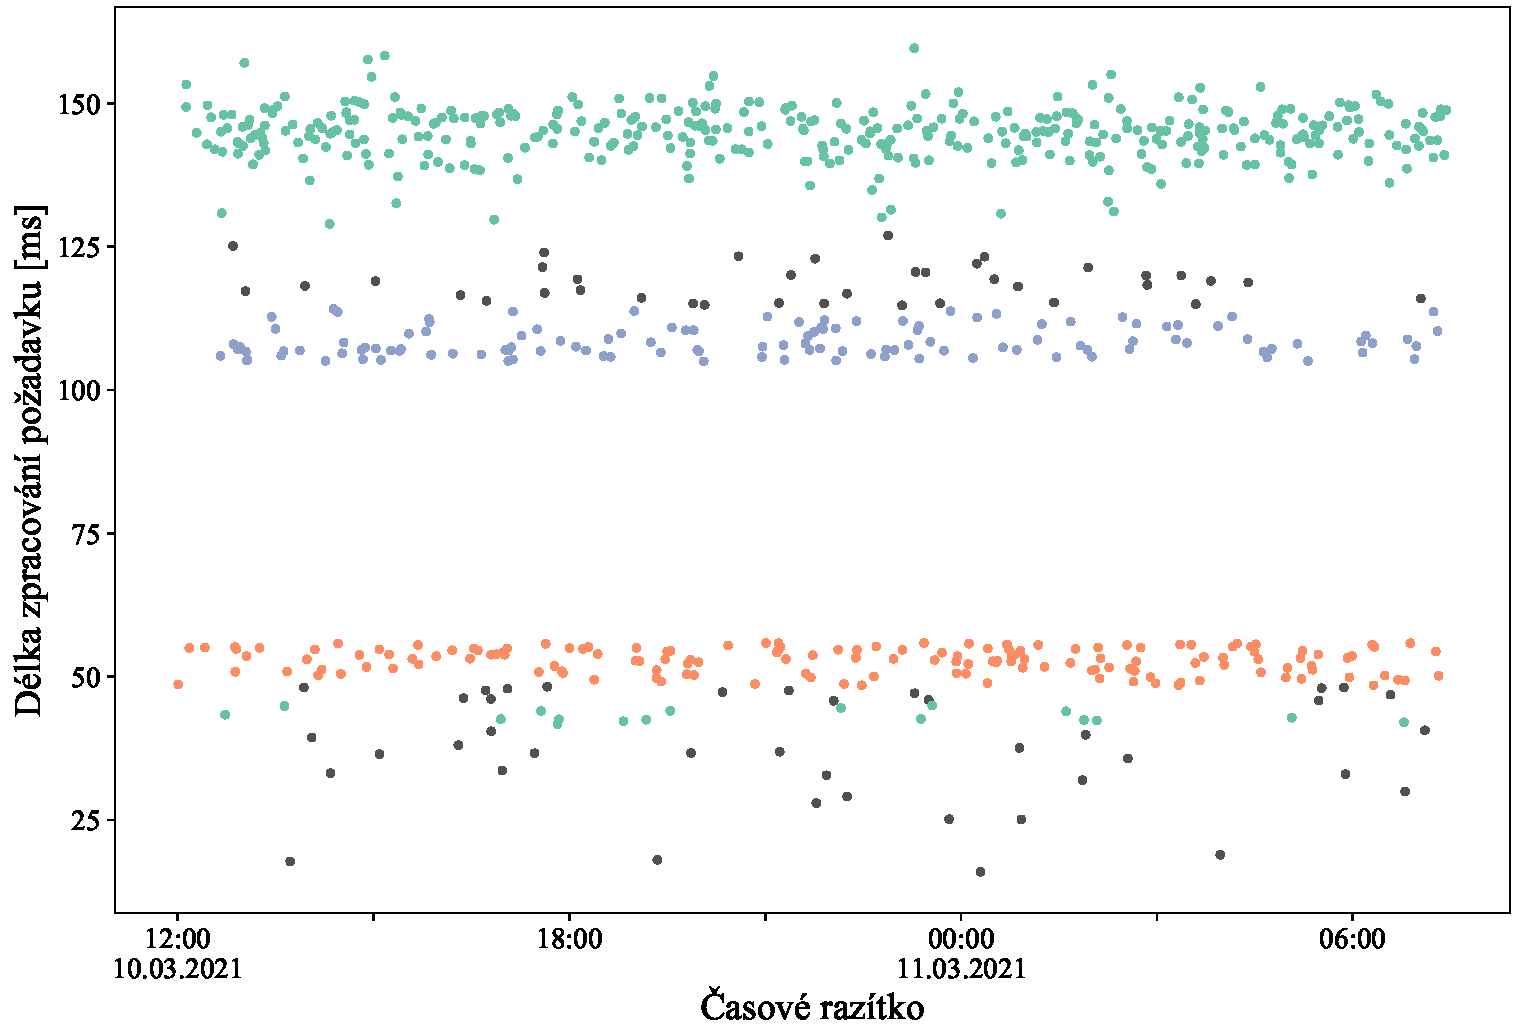
\includegraphics[width=0.84\textwidth]{obrazky/anomaly-detection-merged-clusters.pdf}
    \caption{Výsledek shlukování outlierů po~sloučení blízkých shluků}
    \label{anomaly-detection-merged-clusters-img}
\end{figure}

\subsection{Rozpoznání anomálie mezi shluky outlierů}
Anomálie byla dříve v~práci definována jako shluk outlierů, nicméně prohlásit všechny čtyři shluky z~obrázku~\ref{anomaly-detection-merged-clusters-img} za~anomálie by bylo mylné. Hlavním kritériem pro anomálii je velikost shluku. Shluk je považován za~anomálii, jestliže je větší než určitá mez. Touto je~5~\% celkové velikosti datasetu. Jedná se však o~uživatelsky nastavitelnou hodnotu, neboť udává pouze anomální toleranci a nemá žádný vliv na~samotný výpočet. Nicméně, před kontrolou velikosti shluků je ještě potřeba provést několik úkonů.

Je zcela patrné, že fialový a oranžový shluk z~obrázku~\ref{anomaly-detection-merged-clusters-img} obsahují krajní hodnoty platných dat, které již byly klasifikovány jako outliery. Tyto budou dále označovány jako \uv{přirozené outliery}. Přestože přirozené outliery tvoří shluky a často dostatečně velké na~to, aby byly považovány za~anomálie, o~anomálie se nejedná. Je proto potřeba tyto umět rozpoznat. Každý nalezený shluk je tedy podroben následujícímu testu. Pokud sousedí s~platnými daty, je jim dostatečně blízko a má řídnoucí tendenci, nebo-li počet jeho prvků ubývá se vzdáleností od~platných dat, jedná se o~přirozené outliery a shluk není prohlášen za~anomálii.

Blízkost se sousedstvím se zjistí tak, že se pro~každý prvek shluku vypočítá medián jeho vzdáleností od~ostatních prvků a jako sousedská vzdálenost se použije jejich medián. Dále existuje-li nějaký platný prvek v~této vzdálenosti od~shluku, lze shluk prohlásit za~souseda platných dat. Ověření řídnoucí tendence probíhá ve~dvou krocích. Nejprve se porovná velikost shluku se~stejně širokou oblastí platných dat. Pokud by byl shluk výrazně větší, tak i kdyby jeho prvky řídly v~rámci něj, neřídnou v~porovnání s~platnými daty. Tolerance je nastavena tak, že shluk může být až~2.5krát větší než stejně široká oblast platných dat. Tato volnost je z~toho důvodu, že rozložení zejména menších datasetů nemusí být pravidelné a na~straně platných dat zrovna může být lokální pokles, který však nic neznamená. Ke~konkrétní hodnotě~2.5 se dospělo během testování při~snaze minimalizovat falešné detekce přirozených outlierů za~anomálie. Druhým krokem je test řídnutí v~rámci shluku samotného. Ten se provádí pouze, pokud je shluk dostatečně velký, konkrétně pokud obsahuje alespoň~15 prvků, jinak nelze tuto vlastnost s~dostatečnou jistotou určit. Test používá metodu modifikovaného z-skóre, která každému prvku přiřadí anomální skóre. Vzhledem k~tomu, že je požadováno, aby blíže k~platným datům byl shluk hustší, prvky na~tomto okraji by měly mít nižší skóre, zatímco na~druhém vyšší. Během práce bylo experimentálně zjištěno, že krajní hodnoty rovnoměrného rozložení mají modifikované z-skóre v~rozmezí~1.3 až~1.4. Z~důvodu možnosti mírných výkyvů se tolerance nastavila na hodnotu~1.7. Ve výsledku tedy pokud má krajní hodnota shluku blíže k~platným datům modifikované z-skóre nižší než~1.7, shluk má řídnoucí tendenci, nebo má přijatelné výchylky. Jestliže je toto skóre vyšší, má buď výrazný výkyv, nebo jeho prvky houstnou.

Dalším úkonem před kontrolou velikosti shluků na anomálie je vyhlazení shluků. Anomální horní zelený shluk na~obrázku~\ref{anomaly-detection-merged-clusters-img} obsahuje i několik okolních outlierů, které by již nemusely být jeho součástí. Shluk lze aplikováním modifikovaného z-skóre vyhladit a tím zpřesnit. Princip však funguje i obráceně. Pokud by shlukování nalezlo pouze střed shluku a krajní hodnoty by vynechalo, modifikované z-skóre by shluk rozšířilo alespoň o~část krajních hodnot. V~obou případech modifikované z-skóre opraví a vylepší shluk. V~první řadě je potřeba zjistit, zda-li je žádoucí shluk rozšířit či zúžit. Myšlenka spočívá v~tom, že pokud má shluk výraznou špičku, již zřejmě nepotřebuje rozšíření. Většina dat je totiž ve~špičce, zatímco na~jejích krajích data řídnou a nelze předpokládat další data ve~významném množství. Naopak je-li shluk rovnoměrnější s~pouze mírnou špičkou, zřejmě lze za~hranicemi shluku nalézt další data, jež jsou krajními prvky rozložení shluku.

Prakticky se to provede aplikováním modifikovaného z-skóre na~shluk stejným způsobem jako u~detekce outlierů popsané v~podkapitole~\ref{detekce-outlier}, tedy s~mediánem a mediánem absolutní odchylky daného shluku a hraničním skóre~2.35. Jsou-li nalezeny nějaké outliery nebo je průměr skóre nejlevějšího a nejpravějšího prvku větší než~1.45, tedy přesahující krajní hodnoty rovnoměrného rozložení, ve~shluku je špička, a~proto se bude vyhlazovat. V~opačném případě se shluk bude rozšiřovat. Při~vyhlazování se jako nový shluk použijí pouze platná data shluku po~výše použitém modifikovaném z-skóre. V~případě rozšiřování se shlukem stane výsledek modifikovaného z-skóre s~parametry daného shluku aplikovaném na všechny outliery. Protože shluk je úzký a cílem je ho rozšířit, musí se zvýšit i limit hraničního skóre.
Uvažovalo by-li se, že takovýto zúžený shluk má šířku polovinu normálního rozložení, tedy~1.5 sigma, na~rozptyl daný skórem 2.35 u~plného rozložení by se dosáhlo hodnotou skóre cca~2.9. Během testování dle sekce~\ref{testovani-konkretni-anomalie} se toto upravilo na~hodnotu~2.95.

Po~odstranění shluků s~přirozenými outliery a korekcí zbývajících shluků již zbývá jen porovnat velikost shluků s~anomálním limitem. Pokud je shluk dostatečně velký, jedná se o~anomálii. Obrázek~\ref{anomaly-detection-anomalous-cluster-img} zobrazuje výsledek rozpoznání anomálních shluků a ve~srovnání s~obrázkem~\ref{anomaly-detection-merged-clusters-img} na~něm lze i vidět vyhlazení anomálního shluku. Obrázek~\ref{anomaly-detection-histogram-img} pak formou histogramu znázorňuje celkový výsledek detekce anomálií.

\begin{figure}[hbt]
    \centering
    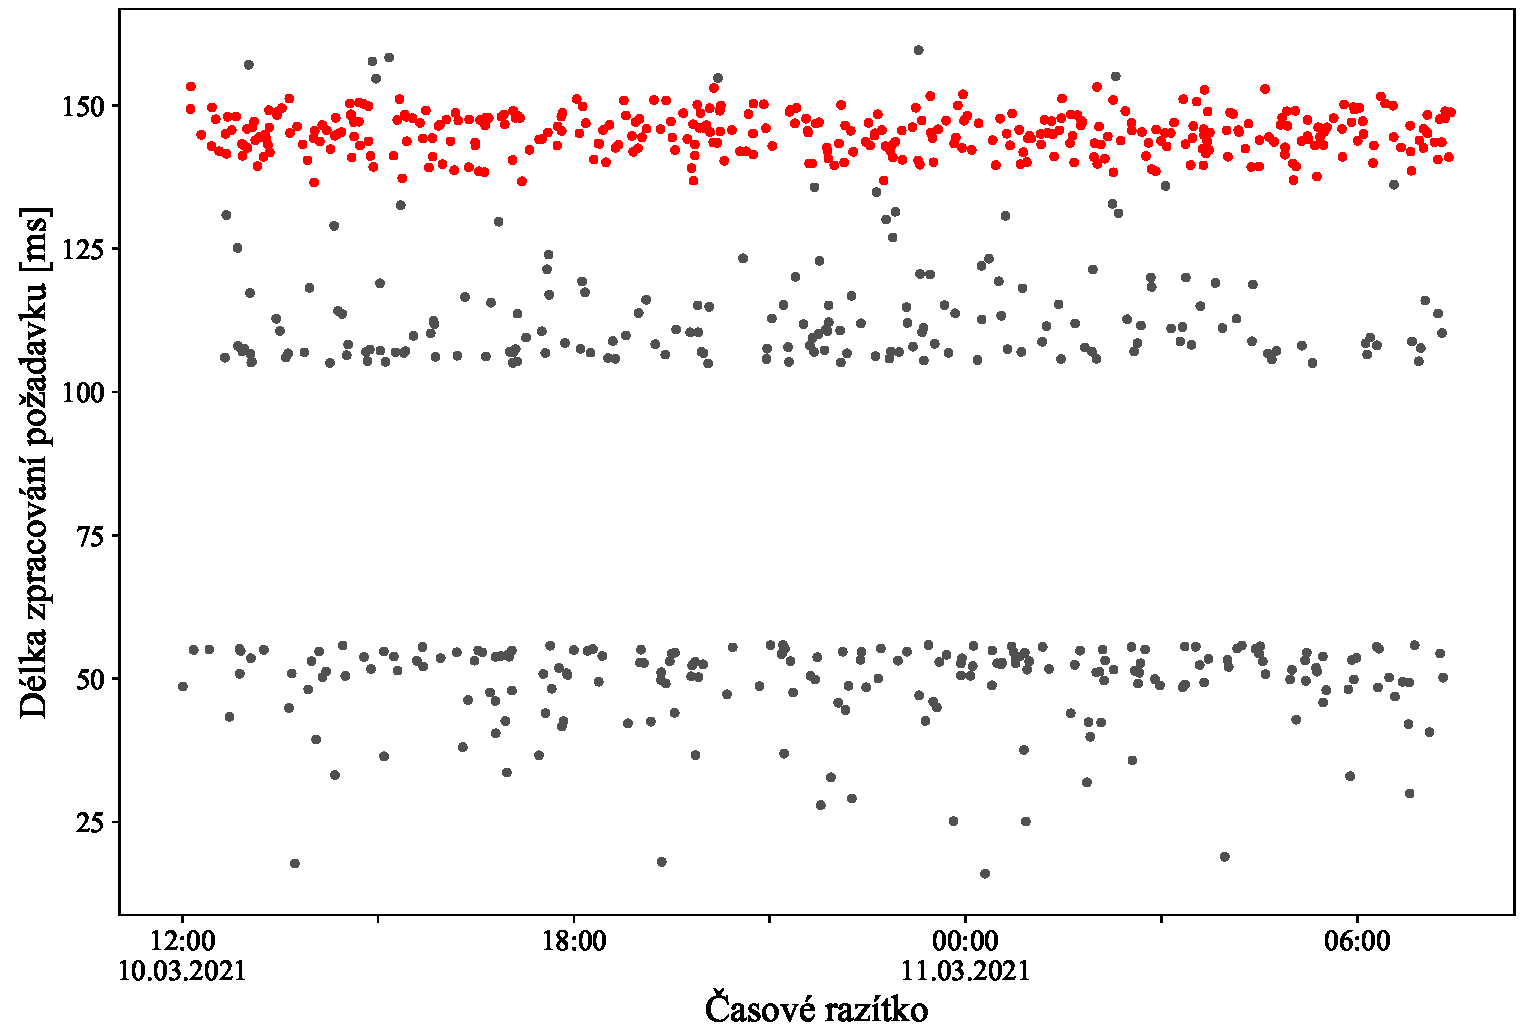
\includegraphics[width=0.935\textwidth]{obrazky/anomaly-detection-anomalous-cluster.pdf}
    \caption{Nalezený anomální shluk mezi shluky outlierů}
    \label{anomaly-detection-anomalous-cluster-img}
\end{figure}

\begin{figure}[!hbt]
    \centering
    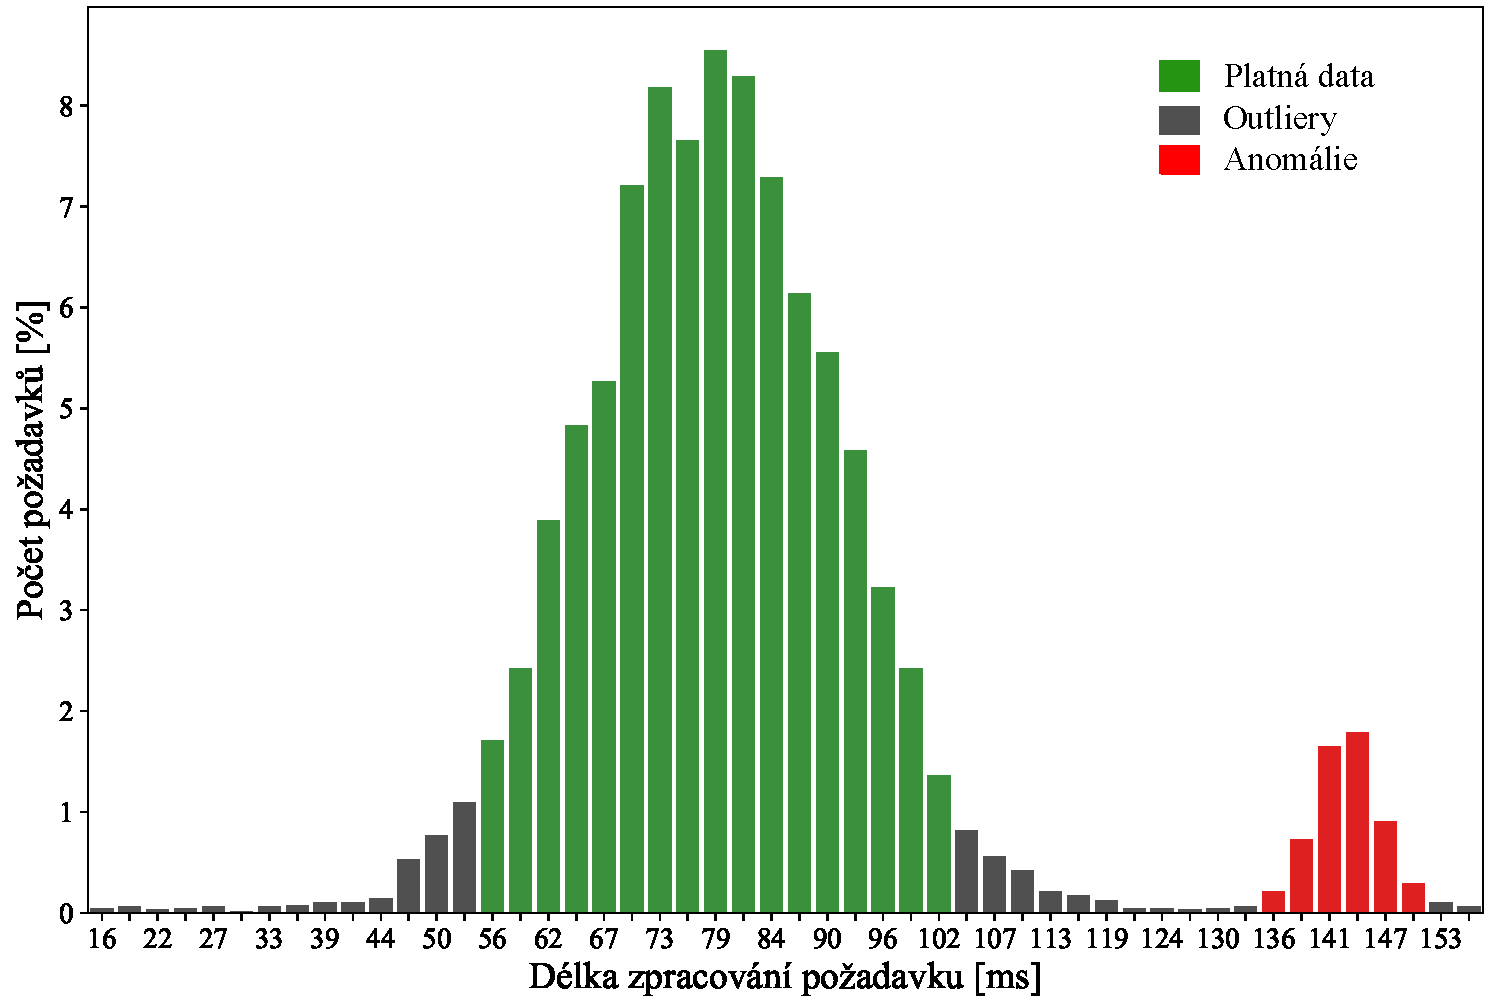
\includegraphics[width=0.935\textwidth]{obrazky/anomaly-detection-histogram.pdf}
    \caption{Celkový výsledek detekce anomálií}
    \label{anomaly-detection-histogram-img}
\end{figure}

Při~práci s~reálnými daty v~RQA systému se ukázalo, že občas je rozptyl délek zpracování požadavků velmi malý, třeba v~jednotkách nebo i zlomcích milisekund. V~tomto případě se i shluk vzdálený jen pár milisekund detekuje jako anomální, neboť relativně ke~zbytku je velmi daleko. Reálně se však jedná skutečně jen o~několik milisekund, což je velmi často zanedbatelné, a~proto může být výhodné umět takové anomálie potlačit. Z~toho důvodu byl zaveden volitelný parametr tolerance, jenž udává, v~jaké vzdálenosti od~platných dat nebudou anomálie detekovány. Prakticky to pouze znamená, že pokud by se měl shluk prohlásit za~anomálii, tak se ještě zkontroluje jeho vzdálenost od~platných dat a jestli je tato menší než daná tolerance, anomálií se nestane.

\section{Detekce anomálií v~chybovosti požadavků}
\label{detekce-anomálii-v-chybach}
Počet chyb během požadavků typicky nabývá hodnoty 0, pokud vše proběhlo v~pořádku, nebo 1 v~případě fatální chyby, která ukončí vykonávání požadavku. Jiné hodnoty se vyskytují pouze u~takových požadavků, které se z~chyb dokáží vzpamatovat. Příkladem může být úspěšná klasifikace obrázku až na~několikátý pokus nebo změna chodu programu po~chybě namísto ukončení.

Hodnoty, s~nimiž se pracuje, jsou tedy celočíselné v~rozmezí 0-N, kde N jsou nízké jednotky. Na~taková data nemá význam shlukování vůbec aplikovat. Místo toho lze použít statistiku, která je mnohem jednodušším i rychlejším řešením. V~podstatě stačí spočítat a porovnat poměry množství chyb v~referenčním datasetu a v~nově příchozích datech. Každá hodnota má nějaké procentuální zastoupení a jestli se toto liší o~více než zvolenou mez, kterou je ve výchozím nastavení hodnota 10~\%, lze to považovat za~anomálii. Podobně je anomálií taková situace, kdy se u~nějakého požadavku vyskytne doposud neviděný počet chyb.

\section{Implementace detekce anomálií}
\label{implementace-detekce-anomalii}
Sekce~\ref{zpracovani-a-ulozeni-dat} zmínila nějakou aplikaci provádějící detekci anomálií. V~sekci~\ref{implementace-sberu-dat} bylo dále uvedeno, že je sběr dat implementován jako knihovna, nikoliv jako specifická spustitelná aplikace. Stejným způsobem je řešena i samotná detekce. Výstupem této práce jsou tedy knihovny použitelné libovolným způsobem. Může tak existovat jedna aplikace, která obstarává sběr dat i detekci, nebo tyto mohou být oddělené. 

Očekávaným vstupem pro~knihovnu jsou buď CSV soubory nebo datové struktury s~již načtenými daty. Knihovna poté data roztřídí na~platné vzory, outliery a anomálie v~případě délek zpracování požadavků nebo u~chybový požadavků pouze určí, zda se jedná o~anomální stav. Knihovna umí i generovat XPlot grafy pro~vizuální zobrazení výsledků.

Detekci anomálií implementuje projekt \emph{AnomalyDetection.Application}, jak již sekce~\ref{implementace-sberu-dat} taktéž naznačila. Není však zcela samostatný a odkazuje na~\emph{AnomalyDetection.Data}, neboť využívá některé jeho třídy. Na~následujícím obrázku~\ref{diagram-zavislosti-trid} je zobrazen diagram závislostí předních tříd podílejících se na detekci anomálií. Neobsahuje pomocné modelové třídy.

\begin{figure}[hbt]
    \centering
    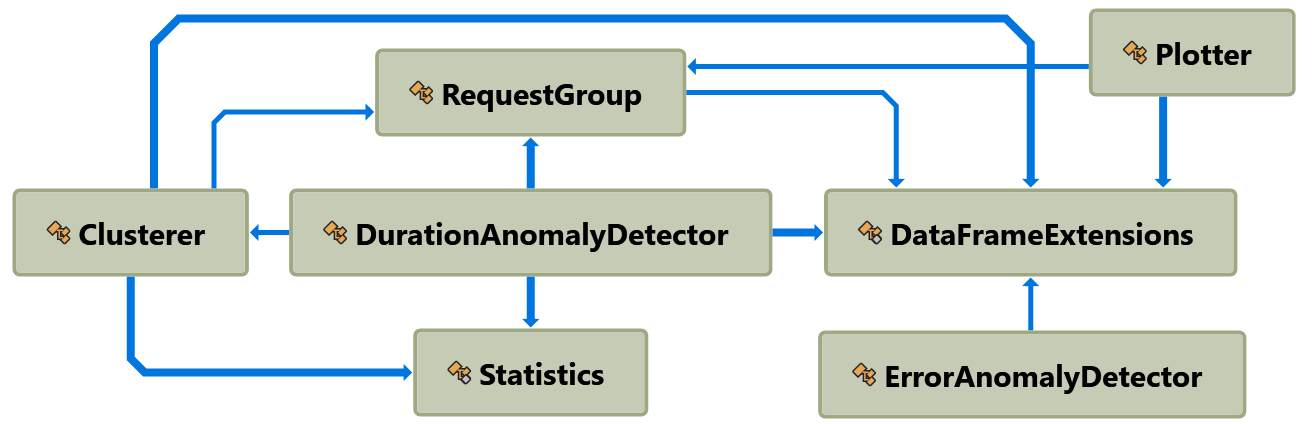
\includegraphics[width=1\textwidth]{obrazky/anomaly-detection-class-dependency-diagram.png}
    \caption{Diagram závislostí tříd ústředních pro~detekci anomálií}
    \label{diagram-zavislosti-trid}
\end{figure}

Analyzovaná data jsou interně reprezentována pomocí dataframů poskytovanými knihovnou \emph{Microsoft.Data.Analysis}. Práce s~nimi ovšem není tak příjemná jako například s~těmi knihovny \emph{Pandas} jazyka Python, a~proto v~projektu existuje třída \texttt{DataFrameExtensions} implementující rozšíření pro~lepší manipulaci s~nimi. Jako kontejner pro~dataframy slouží třída \texttt{RequestGroup}, která zastřešuje všechna data napříč celé analýzy pro~daný typ požadavku určité služby. Obsahuje dataframe zvlášť pro~platná data, outliery, anomálie nebo i mezikroky detekce. Tato data lze vizualizovat pomocí třídy \texttt{Plotter}.

Velký význam pro~detekci anomálií mají statistické výpočty, o~které se stará třída \texttt{Statistics}. Obsahuje metody pro~výpočet modifikovaného z-skóre, mediánu absolutní odchylky, mediánů vzdáleností mezi sousedy nebo i pro generování náhodných čísel.

Další ústřední třídou je \texttt{Clusterer}. Ta implementuje veškeré operace spojené se~shlukováním. Především se jedná o~aplikaci algoritmů DBSCAN a HDBSCAN dostupných z~knihoven \emph{DBSCAN.RBush} a \emph{HdbscanSharp}. Zde stojí za~zmínění, že tato HDBSCAN implementace je v~době psaní práce v~.NET jediná a má značný nedostatek. Vzájemné vzdálenosti bodů jednoduše uchovává ve~2D~poli, oproti například právě DBSCANu, jenž využívá RBush strom. Tím pádem má kvadratickou paměťovou složitost, a nedokáže proto zpracovat velké množství dat. Například dataset o~50 000 prvcích by vyžadoval~\(50 000\times50 000\times8 = 20\)~GB paměti. Dodatečných \(\times8\) proto, že se jedná o~typ \texttt{double}, jenž má velikost 8~B. Naštěstí se HDBSCAN aplikuje pouze na~outliery, které by nikdy neměly dosahovat z~tohoto pohledu nebezpečného množství. Detekce anomálií se totiž bude provádět dostatečně často, aby tak velké datasety ani nevznikaly.

Dále \texttt{Clusterer} obsahuje metody pro~normalizaci výsledků těchto algoritmů. Žádoucí je mít pro~každý bod číselné označení shluku, ke~kterému patří. DBSCAN však vrací kolekci seznamů, kde každý seznam reprezentuje shluk. Výsledek HDBSCANu pak sice je seznam číselných označení pro~každý bod, nicméně tyto nejsou rozumně seřazeny od~nuly, nýbrž se jedná o~čísla uzlů v~kondenzovaném stromu. Po normalizaci mají šumové body přiřazenu hodnotu -1 a ostatní dle příslušnosti ke~shluku 0-N, kde N je počet shluků.

Náročnější na~implementaci se ukázalo být slučování blízkých shluků. Nejprve je nutné seřadit shluky dle hodnot mediánů, aby bylo možné porovnat přímé sousedy. Poté se mezi všemi sousedy otestuje podmínka na slučitelnost, čímž vzniknou dvojice indexů shluků ke~sloučení. Následně se sloučí ty dvojice, které mezi sebou mají tranzitivní vztah, výsledkem čehož jsou seznamy indexů shluků tvořící výsledné shluky. V~posledním kroku se shluky sloučí dle těchto seznamů. V~neposlední řadě \texttt{Clusterer} implementuje kontrolu shluku na~přirozené outliery platných dat.

Za~řízení detekce anomálií mezi délkami zpracování požadavků nese odpovědnost třída \texttt{DurationAnomalyDetector}. Ta ve svém veřejném protokolu zpřístupňuje pouze metody \texttt{FindOutliers()} a \texttt{FindAnomalies()}, které se řídí návrhem z~kapitoly~\ref{detekce-anomalii-v-delkach-pozadavku} a pro~dílčí operace využívají třídy \texttt{Statistics} a \texttt{Clusterer}. Třída \texttt{ErrorAnomalyDetector} pak zase obstarává detekci anomálií v~chybovosti požadavků. Jedná se o~malou třídu s~jedinou metodou \texttt{IsInputAnomalous()}, jež porovnává poměry počtů chyb mezi vstupními a referenčními daty dle sekce \ref{detekce-anomálii-v-chybach} a vrací výsledek typu \texttt{bool}. 

\section{Čištění kolekce dat}
\label{cisteni-kolekce-dat}
Vlastnoruční generování dat přináší několik výhod, jež usnadňují jejich zpracování. Je zaručeno, že žádné hodnoty nebudou chybět. Všechny hodnoty budou správných typů. Neexistují neplatné hodnoty. Vhodný formát potom zaručuje proces popsaný v~kapitole~\ref{sber-dat}. Jediná věc, která se ještě musí zajistit, je odstranění outlierů z~referenčního datasetu. Řešením je provedení navržené detekce outlierů nad~referenčním datasetem. V~datasetu zůstanou pouze platná data a během dalších detekcí se již tato mohou použít pro~určení outlierů.

Během průběžné detekce v~nových datech se pak do~referenčního datasetu budou přidávat opět pouze platná data a ostatní se zahodí. Toto však platí jen pro~detekci mezi délkami zpracování požadavků. U~počtů chyb se budou přidávat i anomální data, neboť tam se pouze ví, že v~daném detekčním okně byla odlišná chybovost, neznají se konkrétní anomální záznamy. To ve~své podstatě ani není možné, pokud se nevyskytne zcela nová chybová třída. Přidávat anomální chybová data však vůbec nevadí. Jedná se totiž o~určitý přirozený vývoj dat. Navíc existuje korelace mezi počtem chyb a délkou zpracování požadavku. Například fatální chyba způsobí, že požadavek bude trvat kratší dobu. Proto je možné, že se zároveň detekují obě anomálie, chybové záznamy patřící i do~anomálie v~délkách zpracování požadavků se nepřidají a tím se poměr chybovosti opět trochu dorovná.